\chapter{The human microbiome and nonalcoholic fatty liver disease}

\section{Introduction}
Non alcoholic fatty liver disease (NAFLD) has been on the rise along with obesity, affecting approximately 25\% of the North American population \cite{preiss2008non}. Most people with NAFLD remain asymptomatic, however, in up to a third of patients NAFLD can progress to nonalcoholic steatohepatitis (NASH), causing inflammation and scarring (fibrosis) in the liver, and decreasing the 5 year survival rate to 67\% \cite{propst1995prognosis}. It is thus important to shed some light on the process by which people progress from NAFLD to NASH to find interventions that prevent NASH.

\subsection{ NASH progression risk}
There are several known genetic and chemical factors that increase the risk of progression to NASH in animal models and humans.

In mice non alcoholic fatty liver disease is often modelled with a methionine/choline-deficient diet (MCD), which induces steatohepatitis in wild type mice. Mice with a toll-like receptor 4 knockout had lower lipid and injury accumulation markers when fed a MCD diet, implying that toll-like receptor 4 has a role in the progression of NAFLD \cite{rivera2007toll}.

In rats liver fibrosis can be induced by dosing with dimethylnitrosamine. Yasuda et al. \cite{yasuda1999suppressive} found that male rats were more prone to this induced liver fibrosis than female rats. Fibrosis biomarkers were reduced when the male rats were dosed with estradiol, and increased when the male rats were additionally given an estradiol-neutralizing antibody. Female rats who had their ovaries removed similarly lost the protective effect \cite{yasuda1999suppressive}. From this, it was concluded that hormones are also a factor in nonalcoholic fatty liver disease progression.

In humans, the I148M variant of the Patatin-Like Phospholipase Domain Containing 3 gene (PNPLA3) correlates with a 3.2 fold increased risk of progression to NASH from NAFLD when homozygous, compared to to patients without the variant \cite{sookoian2011meta}. The heterozygous gene was found to be associated with fatty liver disease in genome wide association studies, but some additional studies have failed to replicate the relationship with NASH \cite{sookoian2011meta}.

On the epigenetic level, many genes are differentially methylated in the livers of patients with advanced NAFLD compared to patients with mild NAFLD. Eleven percent of genes are differentially hypomethylated in advanced NAFLD (compared to 3\% hypermethylated), leading to increased expression \cite{murphy2013relationship}. In advanced NASH specifically, some tissue repair genes were hypomethylated while some metabolism pathways such as 1-carbon metabolism were hypermethylated. However, only 7\% of the differentially methylated genes were found to be differentially transcribed \cite{murphy2013relationship}.

On a metabolite level, Raman et al. found differences in the number of volatile organic compounds detected in patients with NAFLD compared to obese patients without NAFLD \cite{raman2013fecal}. Reactive oxygen species have also been implicated in NASH due to their involvement in the mechanism of steatohepatitis-inducing drugs \cite{berson1998steatohepatitis}.

The microbiome is thought to have an effect on host digestion and absorption of nutrients \cite{gill2006metagenomic}. Anaerobic carbohydrate fermentation produces short chain fatty acids, which make up 10\% of the calories in a Western diet \cite{mcneil1984contribution} Some groups claim a link between ethanol-producing gut bacteria and NAFLD \cite{zhu2013characterization} \cite{jiang2015dysbiosis}, however the evidence was inconclusive since no multiple test correction was performed.

Non alcoholic fatty liver disease is related to obesity, and studies in mice reported that the mouse gut microbiome associated with diet-induced obesity can be transplanted to lean mice and cause them to gain weight while eating the same amount of food \cite{turnbaugh2008diet}. The gut microbiome is an important factor in obesity and potentially obesity related ailments, and its relationship to NAFLD warrants investigation.

\subsection{Data}
Applying next generation DNA sequencing techniques to microbiome research is a relatively new field that has yet to set data analysis standards. There are some considerations that should be made when constructing a data analysis strategy.

\paragraph{Data is multivariate}\mbox{}\\
Experiments of this nature typically have low sample sizes due to budget constraints, sample collection difficulties, patient compliance, and other issues. As a result, the number of taxon or gene function comparisons made are often a magnitude larger than the sample size. This is known in statistics as having more variables than observations, or having fat data. The higher the ratio of variables to observations are, the less likely standard statistical techniques are to be reliable \cite{osborne2004sample}.

At a minimum, researchers should include multiple test corrections to ensure that the results they are reporting are more likely to be reproducible, at the expense of having p-values less than 0.05. Unfortunately many studies have been published in high impact journals without multiple test corrections, including four out of five of the papers in the literature about the gut microbiome and NAFLD (Fig\. ~\ref{nafld_fig1}).

\paragraph{Data is compositional}\mbox{}\\
In both gene tag sequencing and metagenomic sequencing experiments, the data is in the form of a list of counts per feature, with the features composing an aspect of the microbiome for each sample. This is compositional data. The total number of reads yielded by the sequencing platform is often platform-dependant and not biologically relevant.

This constrained sum causes the abundance of different taxa to appear to be negatively correlated with each other when analyzed by conventional statistics \cite{gloor2016s}. When one taxa increases in abundance, the counts detected in other taxa decrease in abundance, even if the taxa are not decreasing in abundance biologically. In addition, correlation and covariance are invalid when calculated from compositional data. Clustering, and dimension reduction are therefore unreliable \cite{lovell2015proportionality}.

Compositional data should be analyzed in a compositional way. In Euclidean space, data points can increase or decrease freely. Compositional data is under a sum constraint, and exist in a non-Euclidean space known as the Aitchison simplex \cite{aitchison1982statistical}. Data transformations such as the centered log ratio can be performed to put the data into Euclidean space, so that it can be analyzed with standard statistical methods that depend on Cartesian coordinates and linear relationships.

However, these techniques are not yet mainstream in the field, resulting in a high number of conclusions made that are not reproducible.

\subsection{Literature}
Several papers have already been published in the literature on the topic of NAFLD and the gut microbiome:

\begin{figure}[h]
\begin{center}
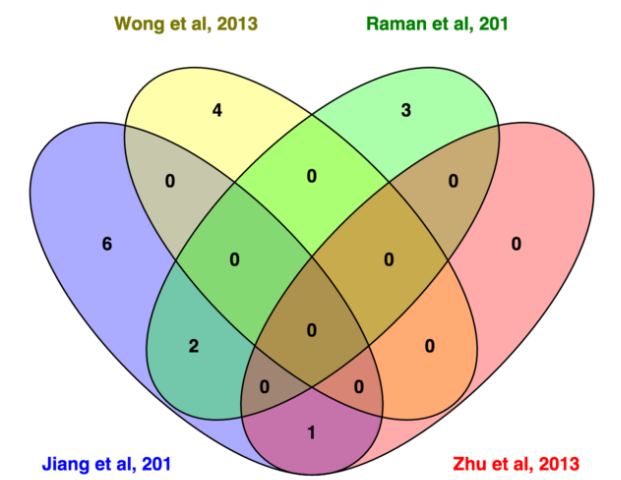
\includegraphics[width=0.7\textwidth]{nafld_papers.png}
\caption[Venn diagram of genera found to be differentially abundant by different studies between NASH/NAFLD and healthy controls.]{\textbf{Venn diagram of genera found to be differentially abundant by different studies between NASH/NAFLD and healthy controls.} Only 3 out of the 16 genera claimed to be differentially abundant were found in two studies: members of the \textit{Escherichia} genus were found in the Zhu \cite{zhu2013characterization} and Jiang \cite{jiang2015dysbiosis} studies, and members of the \textit{Lactobacillus} and \textit{Oscillibacter} genus were found in the Jiang \cite{jiang2015dysbiosis} and Raman \cite{raman2013fecal} studies.}
\label{nafld_fig1}
\end{center}
\end{figure}

Jiang et al, 2015 \cite{jiang2015dysbiosis} compared 53 NAFLD patients with 32 healthy controls. The NAFLD patients had a significantly higher BMI ($P<0.01$). Each sample had an average of 0.6 million reads, from sequencing the V3 region of the 16S rRNA gene on the Illumina sequencing platform. The reads were annotated with the Ribosomal Database Project \cite{cole2009ribosomal}. Differential abundance was determined using Projection on Latent Structures - Discriminant Analysis (PLS-DA) methods, which is not statistically valid when performed on compositional data. They found a relative increase in members of the \textit{Lentisphaerae} phyla and the \textit{Oscillibacter} and \textit{Flavonifractor} genera in the healthy group, and a relative increase in members of the \textit{Clostridium XI}, \textit{Anaerobacter}-related, \textit{Streptococcus}, and \textit{Lactobacillus} genera in the NAFLD group.

Zhu et al, 2013 \cite{zhu2013characterization} compared 16 non-obese controls, 25 obese patients, and 22 NASH patients. All of the patients were pediatric, and the NAFLD group all had a BMI higher than the 85th percentile while the healthy group had BMIs less than the 85th percentile. A 16S rRNA gene tag sequencing experiment was performed and reads were sequenced in a 454 pyrosequencer. This group used MG-RAST \cite{meyer2008metagenomics} and QIIME \cite{caporaso2010qiime} to analyze their data. Note that in the PCoA plot (Figure 1 in \cite{zhu2013characterization}), there is only 11\% variance explained by the first co-ordinate axis, and they had to plot the first co-ordinate axis with the 3rd co-ordinate axis (3\% variance explained) to show the group separation. By comparing the average absolute read count for each taxa in each group, this group found that members of the \textit{Proteobacteria} phylum, the \textit{Enterobacteriaceae} family, and the \textit{Escherichia} genus had significantly higher average counts in NASH patients compared to obese patients and healthy controls.

Raman et al, 2013 \cite{raman2013fecal} compared 30 NAFLD patients with 30 healthy controls. All the healthy controls had a BMI less than 25 while all the NAFLD patients had a BMI greater than 30. The 16S rRNA gene was amplified and sequenced with 454 pyrosequencing, yielding 2000 reads per sample. Reads were annotated with the Ribosomal Database Project \cite{cole2009ribosomal}. UniFrac analysis was performed with QIIME \cite{caporaso2010qiime}, and differential abundance was tested with Metastats \cite{paulson2011metastats}. They found a relative increase in members of the \textit{Lactobacillus}, \textit{Robinsoniella}, \textit{Roseburia}, and \textit{Dorea} genus in NASH patients and a relative increase in members of the \textit{Oscillibacter} in healthy patients.

Wong et al, 2013 \cite{wong2013molecular} compared 16 NASH patients with 22 healthy controls. They amplified the V1-V2 variable region of the 16S rRNA gene with pyrosequencing, yielding 4-11 thousand reads per sample. Reads were clustered with UCLUST \cite{edgar2010search} and annotated with the Ribosomal Database Project \cite{cole2009ribosomal}. Members of the the genera \textit{Parabacteroides} and \textit{Allisonella} were found to be relatively increased in NASH patients, while members of the genera \textit{Faecalibacterium} and \textit{Anaerosporobacter} were relatively increased in healthy controls.

Boursier et al, 2015 \cite{boursier2016severity} compared 30 patients with normal liver fibrosis (stage F0 or F1) to 27 patients with stage F2 or greater fibrosis, 35 of which had NASH A gene tag experiment was performed on the V4 region of the 16S rRNA gene, and sequenced on an Illumina platform, yielding an average of 0.2 million reads per sample. Reads were annotated with the Greengenes database \cite{desantis2006greengenes}, and differential abundance was measured by a Mann-Whitney test. A metagenomic imputation was performed with PiCrust \cite{langille2013predictive}, annotated with KEGG \cite{kanehisa2000kegg}, and analysed with LEfSE \cite{segata2011metagenomic}. A relative increase in members of the \textit{Bacteroides} phylum and a relative decrease in members of the \textit{Prevotella} phylum was found in NASH, compared to healthy controls. From the metagenomic imputation, the gut microbiome of NASH patients was found to be significantly enriched in functional categories related to carbohydrate, lipid, amino acid, and secondary metabolism.

Many of the studies had healthy controls with a lower BMI, so it is difficult to separate whether the differences found are related to NAFLD progression or obesity.

Fig\. ~\ref{nafld_fig1} shows a Venn diagram illustrating the inconsistency of the literature on the gut microbiome and NAFLD. Of these, only Raman et al. \cite{raman2013fecal} reported using a multiple test correction.

Since these five studies do not form a consistent story about the gut microbiome and NAFLD, we conducted own analysis using a compositional data (CoDa) approach with effect size as the primary measure, such that our results are replicable \cite{halsey2015fickle}. Additionally, we generate the first deeply sequenced metagenomic sample set to examine functional capabilities in this disease.

\FloatBarrier

\section{Methods}
In total, 67 samples were collected: 29 from patients with nonalcoholic steatohepatitis (NASH), 14 from patients with simple steatosis (SS), and 24 from healthy controls. The median BMIs were 26.70, 27.34, and 32.06, and the median ages were 36, 49, and 46.5 for healthy, SS, and NASH respectively. A full description of the patient intake, metadata collection, and sample harvesting procedures are provided in Appendix ~\ref{AppB}, written by Hannah Da Silva from Allard research group in Toronto.

DNA extraction was performed with the \href{http://omegabiotek.com/store/product/stool-dna-kit/}{E.Z.N.A.® Stool DNA Kit}, and the protocol was followed with the addition of lysozyme with an extra 30 minute incubation at 37 degrees Celsius, between steps 2 and 3.

\subsection{16S rRNA gene tag experiment}

DNA was amplified by PCR using the Earth Microbiome V4 primer set \cite{caporaso2012ultra}, with the addition of combinatorial in-line barcodes so that all the samples could be sequenced in the same sequencing run \cite{gloor2010microbiome}. The DNA was sequenced on the Illumina MiSeq platform with paired end 220 nucleotide reads, producing 25 million reads in total.

Reads were overlapped with Pandaseq \cite{masella2012pandaseq}, clustered into Operational Taxonomic Units (OTUs) using UCLUST \cite{edgar2010search}, and annotated with the SILVA database \cite{quast2013silva} using mothur \cite{schloss2009introducing}, producing a table of counts per OTU per sample. Twelve million (48\%) of the reads were successfully overlapped and annotated into 232 OTUs, which we have found to be a typical yield for this type of experiment. Differential abundance was analyzed using ALDEx2 \cite{fernandes2014unifying}.

A generalized workflow for processing 16S rRNA gene sequencing reads is available at \url{https://github.com/ggloor/miseq_bin}. The workflow for the 16S rRNA gene tag experiment analysis from the count table stage is on GitHub: \url{https://github.com/ruthgrace/nafld_metaphlan_pca}.

\subsection{MetaPhlAn}

MetaPhlAn (Metagenomic Phylogenetic Analysis) \cite{segata2012metagenomic} is a piece of software that allows one to infer the taxa present based on the metagenomic sequencing experiment. We used this to generate a count table per taxa per sample, and will compare it to our experimental results from the 16S rRNA gene tag sequencing experiment.

The \href{https://bitbucket.org/nsegata/metaphlan/wiki/MetaPhlAn_Pipelines_Tutorial}{MetaPhlAn tutorial} was followed, using an additional \verb|marker_counts| option in the \verb|merge_metaphlan_tables.py| step to produce a count table instead of a relative abundance table. The workflow for the MetaPhlAn analysis from the count table stage is on GitHub: \url{https://github.com/ruthgrace/nafld_metaphlan_pca}.

\subsection{Metagenomic experiment}

\textsc{\begin{table}[!ht]
% \begin{adjustwidth}{-2.25in}{0in} % Comment out/remove adjustwidth environment if table fits in text column.
\begin{tabular}{|l|}
\hline
\bf{Study inclusion criteria}\\ \hline
BMI $>$ 40 kg/m2\\
or BMI $>$ 35-40 kg/m2 with severe weight loss responsive comorbidities,\\
i.e. DM2, hypertension, hyperlipidemia, sleep apnea\\
and/or gastroesophageal reflux disease\\
or physical problems interfering with lifestyle\\
and who have been assessed by the multidisciplinary bariatric team\\
as suitable candidates for laparoscopic RYGB\\ \hline
Male and female\\ \hline
Age 18 years or older\\ \hline
Alcohol consumption $<20$g/d\\ \hline
If known to have hyperlipidemia or DM2,\\
need to be stable drug regimen for at least 3 months prior to study entry\\ \hline
\bf{Study exclusion criteria}\\ \hline
Liver disease of other etiology\\ \hline
Advanced liver disease\\
(need for liver transplantation in one year\\
or complications such as variceal bleeding, ascites or jaundice)\\ \hline
Abnormal coagulation or other reasons contraindicating a liver biopsy\\ \hline
Medications known to precipitate steatohepatitis 6 months prior to entry\\ \hline
Regular intake of non-steroidal anti-inflammatory drugs;\\
prebiotics, probiotics or antibiotics, ursodeoxycholic acid\\
or any experimental drug in the 3 months prior to study entry\\ \hline
Type 1 diabetes\\ \hline
Chronic gastrointestinal diseases\\ \hline
Previous gastrointestinal surgery modifying the anatomy (prior to bariatric surgery)\\ \hline
Smoking\\ \hline
Pregnancy or breastfeeding\\ \hline
Patients not tolerating Optifast,\\
which is a standard weight loss diet given to all patients pre-bariatric surgery\\ \hline
\end{tabular}
\caption[List of overall study inclusion and exclusion criteria.]{ \textbf{List of overall study inclusion and exclusion criteria.} This table lists the inclusion and exclusion criteria for the 16S rRNA gene tag experiment.}
\label{nafld_table_1}
% \end{adjustwidth}
\end{table}}

\textsc{\begin{table}[!ht]
% \begin{adjustwidth}{-2.25in}{0in} % Comment out/remove adjustwidth environment if table fits in text column.
\begin{tabular}{|l|}
\hline
\bf{Study inclusion criteria}\\ \hline
NASH severity\\ \hline
\bf{Study exclusion criteria}\\ \hline
Took antibiotics at any point\\ \hline
Started Optifast diet early\\ \hline
Sample not frozen immediately after collection\\ \hline
Blood glucose over 7.8 mmol/l\\ \hline
\end{tabular}
\caption[List of inclusion and exclusion criteria for metagenomic study.]{ \textbf{List of inclusion and exclusion criteria for metagenomic study.} Patients were selected for the metagenomic study out of the patients selected for the 16S rRNA gene tag sequencing study with the following criteria. Ten healthy and ten patients with NASH were selected in total.}
\label{nafld_table_2}
% \end{adjustwidth}
\end{table}}

A metagenomic sequencing experiment was performed using total bacterial DNA from 10 healthy controls and 10 of the patients with NASH. Samples from healthy patients were selected to exclude confounding factors (Table ~\ref{nafld_table_2}). Samples from NASH patients were selected for the most extreme NASH phenotype, and had higher effect sizes in the 16S rRNA gene tag experiment than the full NASH group.

The DNA was sequenced on the Illumina HiSeq platform, with single end 100 nucleotide reads. Samples were barcoded and sequenced on the same sequencing run. After sequencing, the reads were quality filtered and demultiplexed into reads per individual sample, yielding nearly 2 billion reads in total.

We used a two pronged strategy to annotate the reads:

First, we created a reference library using the inferred taxa from the 16S rRNA gene tag experiment. For each genus observed we randomly picked 10 strain genomes from the NCBI bacterial genome database. For genera with less than 10 fully sequenced representatives, we selected all available genomes. The library was made with 1134 genomes from 104 bacterial genera. The open reading frame (ORF) library was then clustered at 99\% identity for each genus using CD-HIT \cite{li2006cd} to decrease the number of ORFs in the library from 3.5 million to 2.25 million. Annotation was performed by querying the SEED database \cite{overbeek2005subsystems} with the BLAST command line tool \cite{altschul1990basic}, and sequenced reads were mapped onto this ORF library. Out of approximately 2 billion reads total, 58.5 million (30.6\%) were mapped by this method, over 5836 unique SEED hierarchy annotations. This is comparable to the proportion of reads commonly annotated in transcriptomic analysis, where in one data set, 15.5\% of sequenced reads could be matched to a known transcript \cite{celaj2014comparison}. The primary limitation of this method is a lack of annotated bacterial sequences. The code for the \href{https://github.com/ruthgrace/make_functional_mapping_library}{reference library creation} and \href{https://github.com/ruthgrace/mapping_library_annotated_counts}{annotation} is on GitHub.

Second, we assembled the reads per sample de novo using Trinity \cite{haas2013novo}, producing 8,847,816 sequences, and removed sequences that matched our reference library with 90\% identity as determined by BLAST \cite{altschul1990basic}, leaving just under 6 million sequences. Just over three and a half million of these assembled sequences were successfully annotated with the SEED database \cite{overbeek2005subsystems}, and sequenced reads were mapped onto this. Approximately 1.32 billion additional reads were annotated by this method, over 7026 unique SEED hierarchy annotations. The code for the custom assembly pipeline is on \href{https://github.com/ruthgrace/exploring_nafld_assembly}{GitHub}, and described in Appendix ~\ref{AppA}. The data from both prongs was amalgamated into a single table of counts per annotation per sample.

Differential abundance was analyzed using ALDEx2 \cite{fernandes2014unifying}. A full description of the workflow for this process is included in Appendix ~\ref{AppA}.

\subsection{Compositional data analysis}

The count tables from the 16S rRNA gene sequencing experiment and the metagenomic experiment are compositional data. We use the Centered Log Ratio transform \cite{} to put the compositional data in Euclidean space so that it can be analyzed with conventional statistics, for example, principal co-ordinate analysis (Figures ~\ref{nafld_16s_biplot}, ~\ref{nafld_metagenomic_pca}, ~\ref{nafld_metagenomic_carb_pca}, ~\ref{nafld_metagenomic_lipid_pca}, and ~\ref{nafld_metagenomic_amino_pca}).

\FloatBarrier

\section{Results}

\subsection{Data sets}
There were originally three groups of patients within these samples: healthy controls, patients with simple steatosis, and patients who had progressed to non alcoholic steatohepatosis. For the metagenomic experiment, 10 of the healthy controls and 10 of the NASH group were selected, based on clinical criteria (Table ~\ref{nafld_table_2}).

From this, three comparisons can be made: healthy compared to simple steatosis (SS), healthy compared to non alcoholic steatohepatosis (NASH), and healthy compared to the extreme NASH patients chosen for the metagenomic study. The samples used in the healthy vs. extreme NASH comparison had already been chosen for the metagenomic study. The healthy vs. simple steatosis (SS) comparison uses all the samples from healthy patients and patients with simple steatosis. The healthy vs. NASH comparison uses all the samples from healthy patients and patients with NASH. The samples used in the healthy vs. extreme NASH are a subset of the healthy vs. NASH comparison. The sample overlap causes spurious correlations, so the effect size plot has been redone in supporting figure ~\ref{nafld_non_overlapping_16s_effect} with non overlapping samples in the different comparisons.

\subsection{16S rRNA gene tag experiment}

The four most abundant genera detected by 16S rRNA gene sequencing (excluding unclassified bacteria) were: \textit{Bacteroides}, \textit{Faecalibacterium}, \textit{Blautia}, and \textit{Pseudobutyrivibrio} (Fig\. ~\ref{nafld_16s_barplot}).

\begin{figure}[h]
\begin{center}
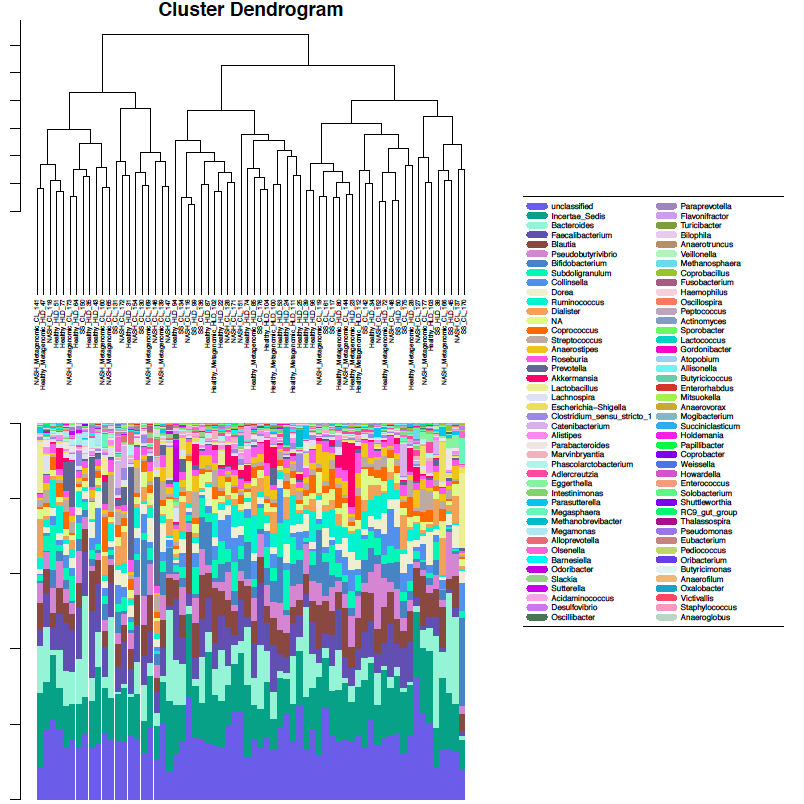
\includegraphics[width=0.95\textwidth]{16s_genus_barplot.png}
\caption[Bar plot of 16S rRNA gene tag sequencing experiment.]{\textbf{Bar plot of 16S rRNA gene tag sequencing experiment.} Each column of this bar plot represents one sample, and each color represents one bacterial genus. Genus names are listed in the legend in order of decreasing total abundance across all samples. Samples do not cluster according to their condition (healthy, simple steatosis, or nonalcoholic steatohepatitis). Note that OTUs that mapped to unclassified or \textit{Incertae Sedis} were removed, and these made up just over a third of the total abundance. This operation is valid in compositional data analysis since it is the rato between OTUs that is measured, but not in non-compositional approaches where the apparent abundance is examined.}
\label{nafld_16s_barplot}
\end{center}
\end{figure}

Figure ~\ref{nafld_16s_barplot} has both a dendrogram and a bar plot. The dendrogram is the result of unsupervised clustering on the centered log ratio transformed values of the 16S rRNA count table. The samples from the different groups (healthy, simple steatosis, and non alcoholic steatohepatitis) are scattered and do not cluster together. The bar plot shows the composition of each sample. Each bar represents one sample, and each color represents one genus. Visually there is no obvious difference in the sample compositions of the different groups.

Unlike the one dimensional representation of the data in the dendrogram, figure ~\ref{nafld_16s_biplot} shows the data in two dimensions, in the form of a principal component analysis (PCA) plot. This plot is variance-based, and shows the samples and OTUs on the same scale. The closer points are to each other, the tighter their correlation. For example, samples CL\_154 and CL\_147 are in close proximity on the plot, so one would expect them to have similar compositions. Genera \textit{Lactobacillus} and \textit{Desulfovibrio} are close, and would be expected to have similar abundances in the different samples. The data is actually multi-dimensional, and the variance explained by each axis is shown in the Scree plot. In a well separated data set, most of the variance would be accounted for by the first two component axis. In this data set the samples are not well separated, and the first two component axis explain just over 20\% of the total variance.

Figure ~\ref{nafld_pcoa} shows a principal co-ordinate analysis (PCoA) on four UniFrac differences. The first is unweighted UniFrac, which is able to distinguish differences between groups stemming from the presence or absence of taxonomic groups. The second is weighted UniFrac, which incorporates phylogenetic information with abundance. The third is information UniFrac, which can separate groups with different abundance profiles (for example, samples where one taxa is dominant, compared to samples that have more even abundances). The fourth is ratio UniFrac, which can separate groups with taxa that are outliers above the baseline abundance. Based on these methods, there are no obvious outliers in this data set - the data is just not well separated.

No obvious structure or separation is evident from the unsupervised clustering on the centered log ratio transformed values in Fig. ~\ref{nafld_16s_barplot}, the principal co-ordinates analysis in Fig. ~\ref{nafld_pcoa} or the principal component analysis in Fig. ~\ref{nafld_16s_biplot}. Furthermore the variance explained by each principal component or co-ordinate axis is not notably high, indicating a rather uniform data set.

To examine individual taxa, ALDEx was used (Fig. ~\ref{nafld_fig3}). This plot shows the difference between groups with the dispersion within groups. Each plot represents one OTU, and OTUs that are rare have a black dot on top. OTUs with a difference between groups that is much higher than the dispersion within groups are significantly differentially abundant. In figure ~\ref{nafld_fig3} no taxa in either of the three comparisons (healthy vs. SS, healthy vs. NASH, or healthy vs. extreme NASH) are significantly differentially abundant.

Table ~\ref{nafld_consistent_otu_table} show which OTUs were consistently differentially abundant (absolute effect size greater than $0.4$) in non alcoholic fatty liver disease or health. In the ALDEx analysis, the taxa consistently abundant in non alcoholic fatty liver disease are circled red, while taxa consistently abundant in the healthy condition are circled black (Figure ~\ref{nafld_fig3}). Note that they are not rare in either of the comparisons (OTUs with low counts are marked with a black dot). These OTUs may have a contributory effect or a protective effect (Table ~\ref{nafld_consistent_otu_table}) on the progression of non alcoholic fatty liver disease.

\begin{figure}[h]
\begin{center}
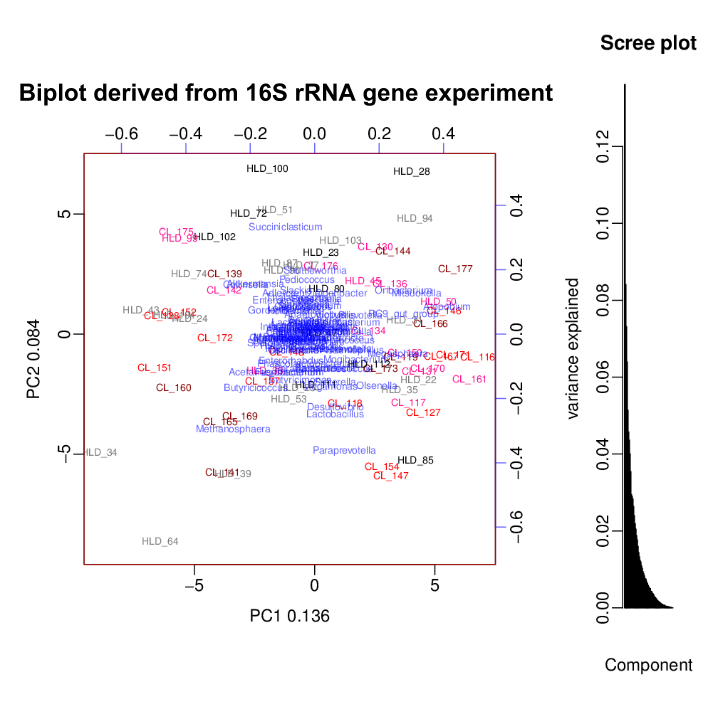
\includegraphics[width=0.95\textwidth]{nafld_16s_biplot.png}
\caption[16S rRNA gene tag sequencing experiment biplot.]{\textbf{16S rRNA gene tag sequencing experiment biplot.} Exploratory analysis using compositional data techniques is done by transforming the counts with the centered log ratio transform, and then performing a principal component analysis. The variance explained by each genus is overlaid on the same principal component analysis plot. Note that the variance explained by the first and the second component is 13.6\% and 8.4\% respectively, indicating that there is not a clear unidirectional separation between groups. Samples from healthy controls selected for the metagenomic study are colored black and prefixed with `HLD' while samples from patients with extreme NASH are colored dark red and prefixed with `CL'. The remaining healthy controls are colored gray, and the remaining NASH samples are colored bright red. Samples from patients with simple steatosis (SS) are colored pink.}
\label{nafld_16s_biplot}
\end{center}
\end{figure}

\begin{figure}[h]
\begin{center}
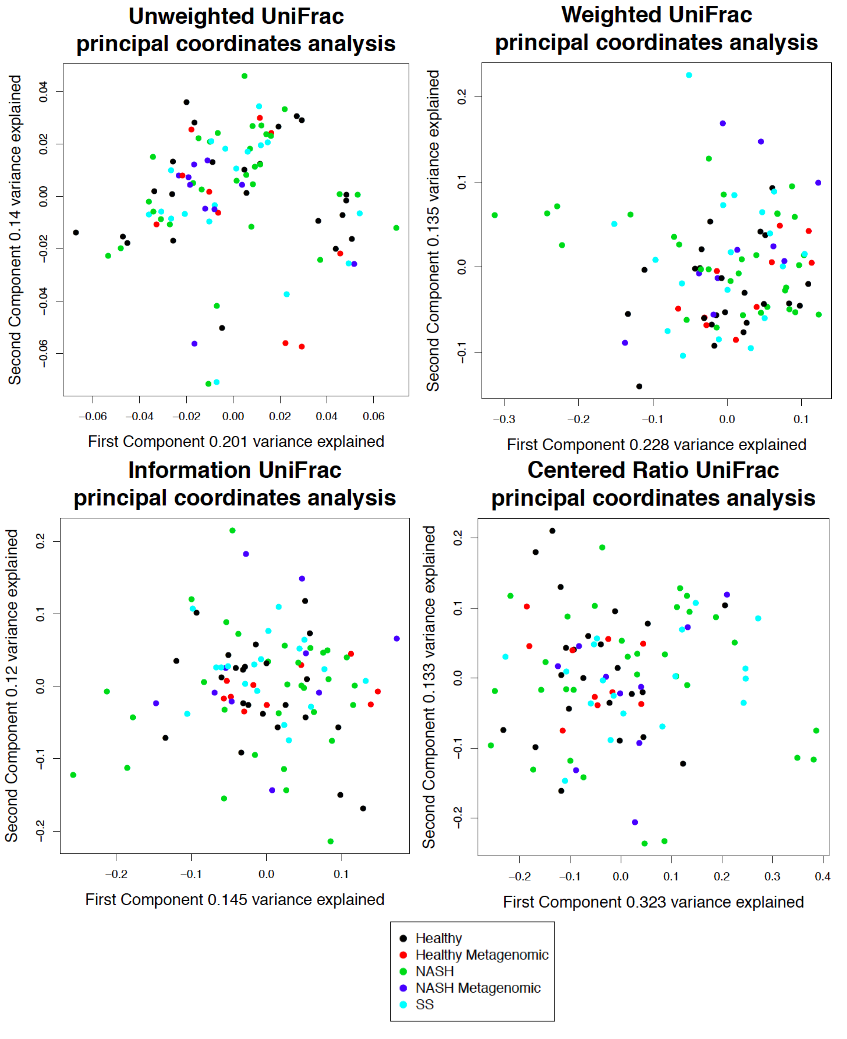
\includegraphics[width=0.95\textwidth]{nafld_16s_pcoa.png}
\caption[Principal co-ordinate analysis of 16S rRNA gene tag sequencing data with different UniFrac weightings.]{\textbf{Principal co-ordinate analysis of 16S rRNA gene tag sequencing data with different UniFrac methods.} Each point represents one sample, and the distances between the samples have been calculated using different UniFrac metrics, taking into account phylogenetic as well as abundance information. There is no obvious separation between groups by any of the UniFrac weightings. Furthermore the variance explained by each principal co-ordinate axis is not notably high, indicating a rather uniform data set, and no samples were observed to be outliers.}
\label{nafld_pcoa}
\end{center}
\end{figure}

\begin{figure}[h]
\begin{center}
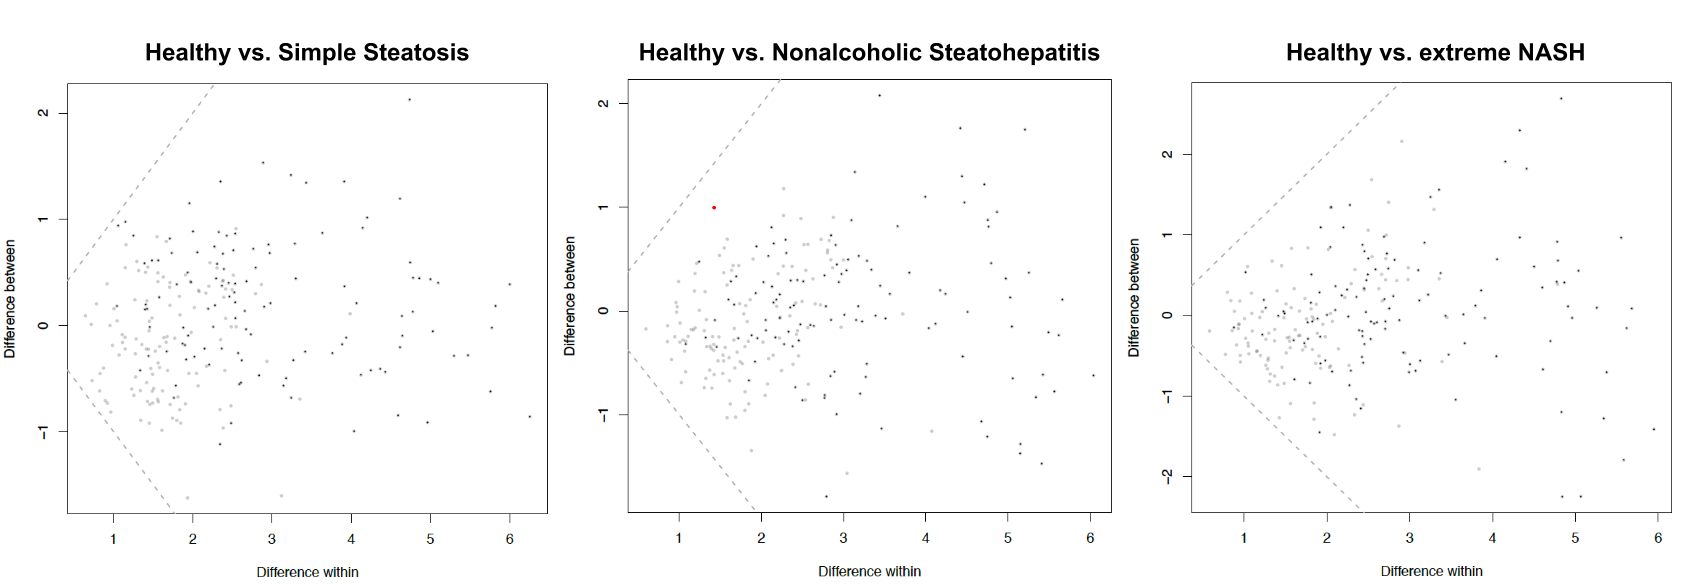
\includegraphics[width=0.95\textwidth]{nafld_16s_aldex.png}
\caption[Effect plot showing difference within vs. difference between groups.]{\textbf{Effect plot showing difference within vs. difference between groups.} Each point represents one OTU, and the dispersion of that OTU within groups is plotted against the difference in abundance between groups. None of the OTUs are more different between groups than within groups. The healthy samples used for these comparisons are the 10 healthy samples used for the metagenomic study. The extreme NASH samples used for these comparisons are the subset of the NASH patients selected for the metegenomic study. The dashed lines represent where the difference in abundance between groups and within group dispersion are equal. Points with a black dot represent OTUs that are rare. Points with a red circle are the top consistently abundant OTUs in non alcoholic fatty liver disease from Table ~\ref{nafld_consistent_otu_table}. Points with a black circle are the top consistently abundant OTUs in the healthy condition from Table ~\ref{nafld_consistent_otu_table}.}
\label{nafld_fig3}
\end{center}
\end{figure}

The Toronto patient population is very diverse, including patients coming from different cultural backgrounds who consume different diets. With this kind of population and diversity, it can be difficult to have sufficient power to detect significant differences. The previous figures ~\ref{nafld_16s_barplot}, ~\ref{nafld_16s_biplot}, ~\ref{nafld_pcoa}, and ~\ref{nafld_fig3} taken together indicate no large difference between groups. We explore effect sizes, since these are known to be more robust and predict the p-values \cite{halsey2015fickle}. Effect size is a standardized difference between means. One common effect size measure is a z-score, which is a difference in means divided by the average standard deviation. In the measure used here, the difference between groups is the median of the signed difference between pairs of points, where one point is in one group, and one point is in the other group. The difference within groups is the median of the absolute difference of pairs of points within a group. The effect size is the ratio of the difference between groups to the difference within groups. In the ALDEx differential abundance test, multiple Monte Carlo instances are sampled across a Dirichlet distribution to estimate technical variance, and the effect size is calculated as the median of the ratio of the between/within differences, across all replicates.

\begin{table}[!ht]
% \begin{adjustwidth}{-2.25in}{0in} % Comment out/remove adjustwidth environment if table fits in text column.
\begin{tabular}{|l|l|l|l|l|l|l|l|}
\hline
\bf{OTU family} & \bf{OTU genus} & \bf{SILVA} &\bf{H Vs. SS} & \bf{H Vs. NASH} & \bf{H vs. extreme} \\
& & \bf{bootstrap} & \bf{effect sizes} & \bf{effect sizes} & \bf{NASH effect} \\
& & \bf{value} & & & \bf{sizes}\\ \hline
Lactobacillaceae & Lactobacillus & 97 & $0.479$ & $0.591$ & $0.898$ \\ \hline
Lachnospiraceae & Blautia & 85 & $-0.413$ & $-0.415$ & $-0.519$ \\ \hline
Bacteroidaceae & Bacteroides & 100 & $-0.657$ & $-0.524$ & $-0.526$ \\ \hline
Ruminococcaceae & Faecalibacterium & 100 & $-0.593$ & $-0.402$ & $-0.549$ \\ \hline
Lachnospiraceae & Incertae_Sedis & 85 & $-0.523$ & $-0.404$ & $-0.682$ \\ \hline
Lachnospiraceae & Dorea & 100 & $-0.628$ & $-0.455$ & $-0.731$ \\ \hline
\end{tabular}
\caption[Top decile of OTUs consistently relatively increased based on effect size from healthy vs. extreme NASH comparison.]{ \textbf{Top decile of OTUs consistently relatively increased based on effect size from healthy vs. extreme NASH comparison.} This table lists the OTUs and their effect sizes in all the comparisons. The OTUs were picked by open reference, by clustering and comparison with the SILVA database \cite{quast2013silva}. Positive effect sizes indicate that the feature was found to be relatively increased in NASH while negative effect sizes indicate that the feature was found to be relatively increased in healthy. OTUs were annotated with SILVA, and a confidence percentage is reported based on the provided bootstrapping algorithm. The 106 OTUs with effect sizes in the top deciles of the healthy vs. extreme NASH comparison were filtered to only include OTUs that had an absolute effect size greater than 0.4 in all comparisons. The tables with all 53 OTUs in each of the top deciles are in supporting figures ~\ref{nafld_top_otu_table} and ~\ref{nafld_bot_otu_table}.}
\label{nafld_consistent_otu_table}
% \end{adjustwidth}
\end{table}

\begin{figure}[h]
\begin{center}
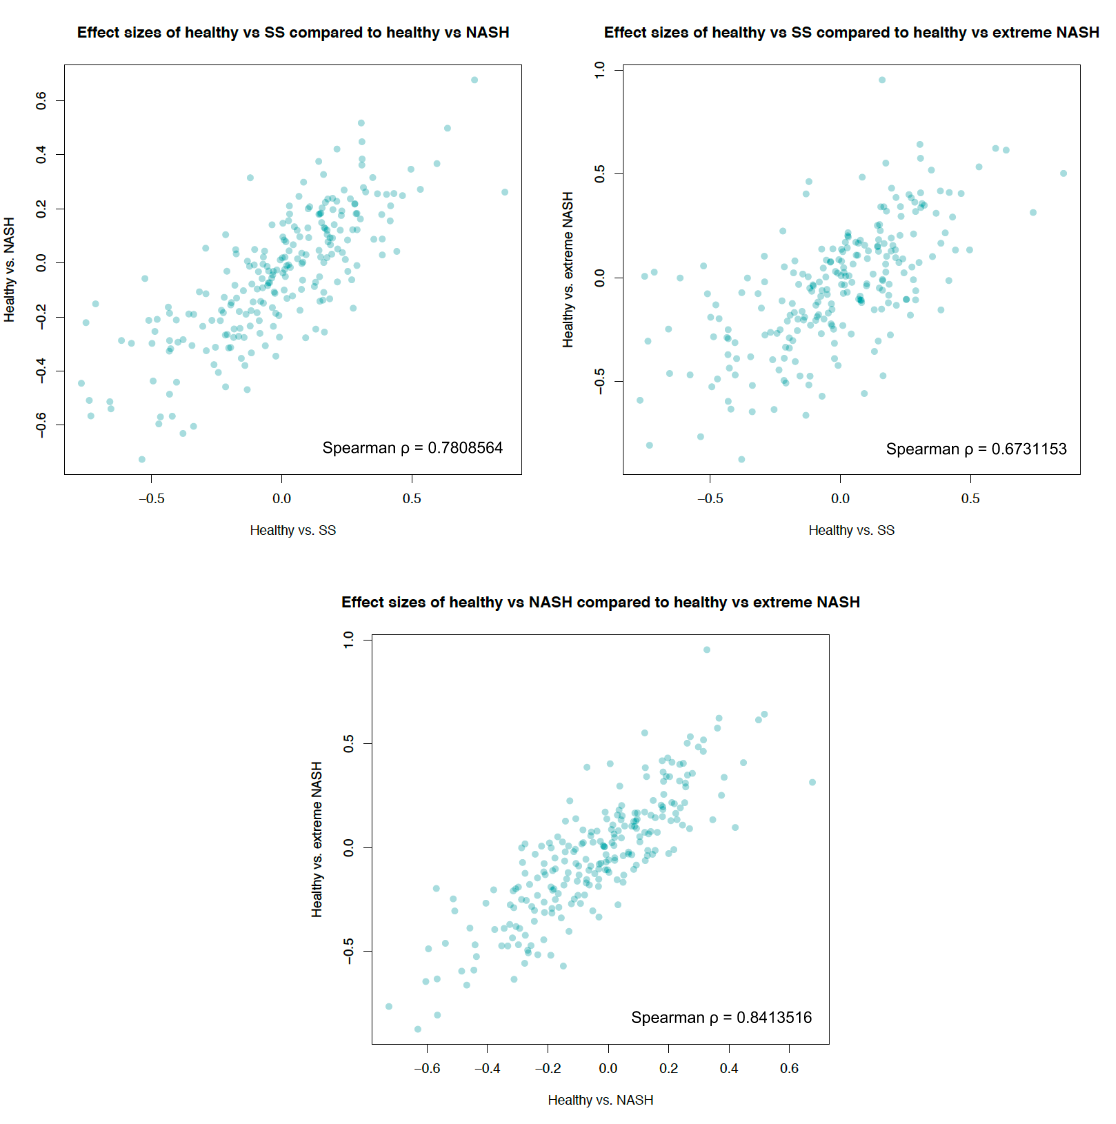
\includegraphics[width=0.9\textwidth]{nafld_16s_effect_sizes.png}
\caption[Correlation in effect sizes of different group experiments.]{\textbf{Correlation in effect sizes of different group experiments.} Each point represents one OTU, and the effect size of that OTU in one comparison (for example, comparing the gut microbiome of healthy patients with patients who have simple steatosis) is plotted against the effect size of that OTU in another comparison. The healthy samples used for these comparisons are the 10 healthy samples used for the metagenomic study. The extreme NASH samples used for these comparisons are the subset of the NASH patients selected for the metegenomic study. The top decile of OTUs relatively increased in NASH for the metagenomic experiment are colored pink (Table ~\ref{nafld_top_otu_table}), and the top decile of OTUs relatively increased healthy for the metagenomic experiment are colored blue (Table ~\ref{nafld_bot_otu_table}). The median difference in the effect sizes of the `Healthy vs. NASH' - `Healthy vs. SS' is 0.062 for the pink points, and -0.0097 for the blue points. The median difference in the effect sizes of the `Healthy vs. extreme NASH' - `Healthy vs. SS' is 0.33 for the pink points, and -0.30 for the blue points. The median difference in the effect sizes of the `Healthy vs. extreme NASH' - `Healthy vs. NASH' is 0.28 for the pink points, and -0.25 for the blue points. }
\label{nafld_fig4}
\end{center}
\end{figure}

\FloatBarrier

Figure ~\ref{nafld_fig4} shows the correlation of effect sizes per OTU, between each comparison. The top deciles of OTUs relatively abundant in the healthy or the extreme NASH condition are colored. If there were truly no effect, then there would be no correlation between the effect sizes for each OTU in the different comparisons. However, in Figure ~\ref{nafld_fig4}, we show that the effect sizes for each OTU in each comparison are correlated. The effect sizes are higher in the Healthy vs. extreme NASH compared to the Healthy vs. SS or Healthy vs. NASH comparison at the extreme deciles. Even though there are no significantly differentially abundant OTUs, the correlation shows that the difference from the healthy baseline are moving in the same direction through SS to NASH to extreme NASH.

When comparing all the healthy samples with all the NASH samples, the genera with the highest effect sizes were \textit{Lactobacillus}, which was relatively abundant in the NASH condition, as well as \textit{Alistipes}, and \textit{Bacteroides}, which were relatively abundant in the healthy condition. However, when only the select 10 healthy samples and the 10 extreme NASH samples used in the metagenomic study are compared (the healthy vs. extreme NASH comparison), the genera with the highest effect sizes are \textit{Phascolarctobacterium} and \textit{Paraprevotella}, which were relatively abundant in the extreme NASH condition, and \textit{Ruminococcus}, which was relatively abundant in the healthy condition.

This corresponds with the qPCR experiment, where \textit{Bacteriodetes}, \textit{Prevotella}, and \textit{Ruminococcus} were tested. Only \textit{Ruminococcus} was found to be significantly differentially abundant, in healthy controls (Anastasia Teterina, personal communication, March 16, 2016).

These results suggest that members of the \textit{Alistipes}, \textit{Bacteroides}, and \textit{Ruminococcus} genera may play a protecting role against NASH progression in the gut microbimoe of healthy patients, and be useful in probiotic therapies. It is possible that members of the \textit{Lactobacillus}, \textit{Phascolarctobacterium}, and \textit{Paraprevotella} genera may be a contributing factor to NASH progression.

\FloatBarrier

\subsection{Metagenomic experiment}

\paragraph{Functional analysis}\mbox{}\\
The sequencing platform yielded 2.8 billion reads. Out of these, 1.3 billion were annotated across 7026 SEED subsystem functional annotations. The SEED subsystems are functional categorizations of gene sequences \cite{overbeek2005subsystems}. The most descriptive and specific SEED subsystem is subsystem 4. Each read is categorized into at most one subsystem 4. Subsystems 1, 2, and 3 are broader, and a read can be categorized into multiple higher categories. We use ALDEx to test for differential expression at the subsystem 4 categorization level (Fig. ~\ref{nafld_metagenomic_aldex}). Because the reads do not have unique categorizations at the higher levels, we use stripcharts to examine these in a descriptive manner (Fig. ~\ref{nafld_metagenomic_subsys1}).

\begin{figure}[h]
\begin{center}
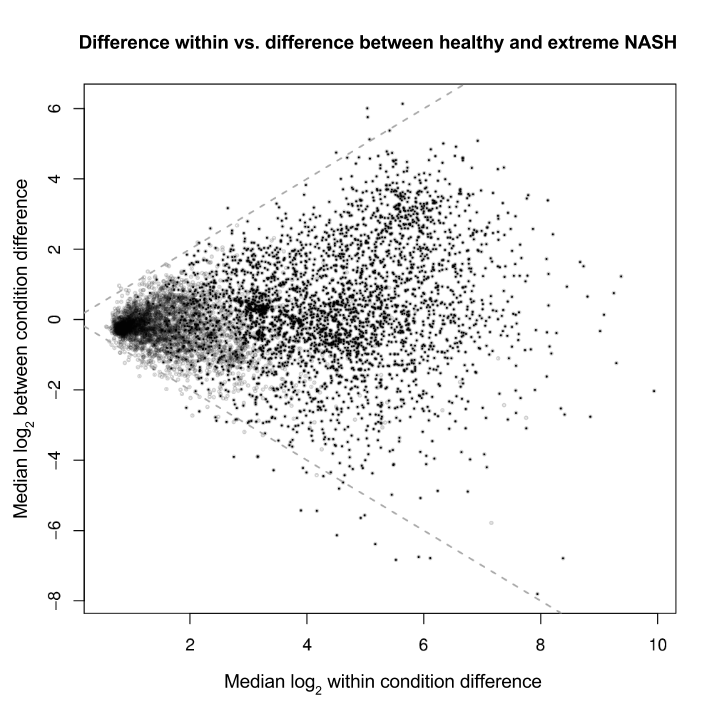
\includegraphics[width=0.95\textwidth]{metagenomic_aldex.png}
\caption[Difference within vs. difference between healthy and extreme NASH for metagenomic data.]{\textbf{Difference within vs. difference between healthy and extreme NASH for metagenomic data.} Each point on this plot represents a functional annotation at the SEED subsystem 4 level. None of the subsystem 4 functional annotations have a significantly greater abundance between groups than within groups.}
\label{nafld_metagenomic_aldex}
\end{center}
\end{figure}

\begin{figure}[h]
\begin{center}
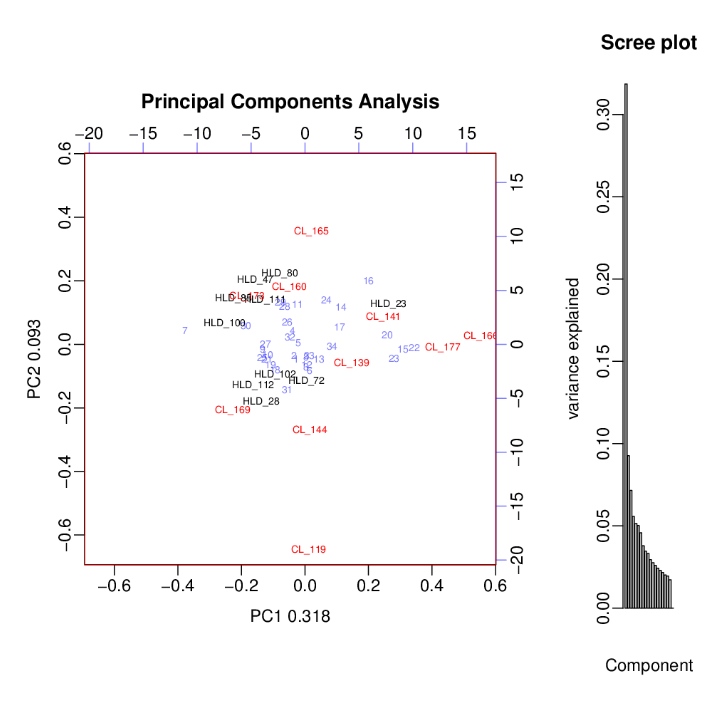
\includegraphics[width=0.95\textwidth]{metagenomic_pca.png}
\caption[Principal components analysis of metagenomic data.]{\textbf{Principal components analysis of metagenomic data.} In this biplot, the healthy samples are shown in black, while the extreme NASH samples are shown in red. Samples CL\_119, CL\_139, CL\_160, and CL\_165 have a steatosis grading of 3. Samples CL\_141, CL\_144, CL\_169, CL\_173, and Cl\_177 have a steatosis grading of 2. Sample CL\_166 has a steatosis grading of 1. The steatosis grading does not appear to separate the samples. The location of the subsystem 4 labels (in blue) show which direction they pull the samples in, in terms of variance. The biplot shows only the thirty four subsystem 4 categories with an effect size greater than 1, out of 7026 categories in total. The key for the subsystem 4 labels is Table ~\ref{nafld_subsys4_labels}. The Scree plot indicates that about 40\% of the variation in the data set was explained by the first two components, and the data is well spread.}
\label{nafld_metagenomic_pca}
\end{center}
\end{figure}

\begin{table}[!ht]
\begin{tabular}{|l|l|}
\hline
\bf{Function ID} & \bf{Function name}\\ \hline
1 & DNA topoisomerase III (EC 5.99.1.2) \\ \hline
2 & 3-oxoacyl-[acyl-carrier protein] reductase (EC 1.1.1.100) \\ \hline
3 & 2-hydroxy-3-oxopropionate reductase (EC 1.1.1.60) \\ \hline
4 & Imidazolonepropionase (EC 3.5.2.7) \\ \hline
5 & Flagellar basal-body rod modification protein FlgD \\ \hline
6 & HflC protein \\ \hline
7 & Diaminobutyrate-pyruvate aminotransferase (EC 2.6.1.46) \\ \hline
8 & Metal-dependent hydrolases of the beta-lactamase \\
& superfamily II \\ \hline
9 & pyoverdine-specific efflux macA-like protein \\ \hline
10 & Homoserine O-acetyltransferase (EC 2.3.1.31) \\ \hline
11 & Threonine kinase in B12 biosynthesis \\ \hline
12 & Molybdopterin biosynthesis protein MoeB \\ \hline
13 & D-allose kinase (EC 2.7.1.55) \\ \hline
14 & Gluconate permease, Bsu4004 homolog \\ \hline
15 & 2-methylisocitrate dehydratase (EC 4.2.1.99) \\ \hline
16 & Uncharacterized protein ImpH/VasB \\ \hline
17 & Phosphate starvation-inducible ATPase PhoH \\
& with RNA binding motif \\ \hline
18 & Spore germination protein GerLC \\ \hline
19 & Phosphohistidine phosphatase SixA \\ \hline
20 & Glutathione-regulated potassium-efflux system \\
& ancillary protein KefG \\ \hline
21 & Histidyl-tRNA synthetase, archaeal-type paralog (EC 6.1.1.21) \\ \hline
22 & 3-hydroxydecanoyl-[acyl-carrier-protein] dehydratase (EC 4.2.1.60) \\ \hline
23 & FKBP-type peptidyl-prolyl cis-trans isomerase slpA (EC 5.2.1.8) \\ \hline
24 & 3-oxoacyl-[ACP] synthase \\ \hline
25 & IncW plasmid conjugative relaxase protein TrwC (TraI homolog) \\ \hline
26 & CO dehydrogenase iron-sulfur protein CooF (EC 1.2.99.2) \\ \hline
27 & Transcriptional regulator of AraC family, \\
& enterobactin-dependent, predicted \\ \hline
28 & Antitoxin YgiT \\ \hline
29 & acyl-acyl carrier protein synthetase (EC 6.2.1.20) \\ \hline
30 & Outer membrane protein GumB, \\
& involved in the export of xanthan \\ \hline
31 & C3 family ADP-ribosyltransferase (EC 2.4.2.-) \\ \hline
32 & Hypothetical SAV0786 homolog in superantigen-encoding \\
& pathogenicity islands SaPI \\ \hline
33 & Predicted cellobiose ABC transport system, \\
& sugar-binding protein \\ \hline
34 & Lipoprotein Bor \\ \hline
\end{tabular}
\caption[Subsystem 4 label key for Figure ~\ref{nafld_metagenomic_pca}.]{ \textbf{Subsystem 4 label key for Figure ~\ref{nafld_metagenomic_pca}.} This table lists the subsystem 4 labels and corresponding names.}
\label{nafld_subsys4_labels}
% \end{adjustwidth}
\end{table}

\begin{figure}[h]
\begin{center}
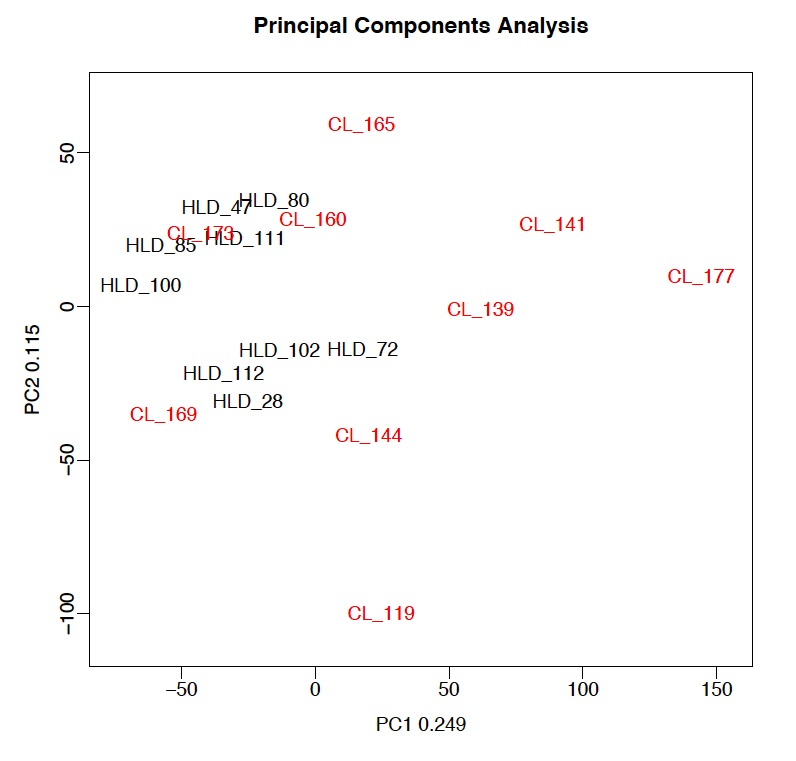
\includegraphics[width=0.95\textwidth]{metagenomic_pca_no_outliers.png}
\caption[Principal components analysis of metagenomic data.]{\textbf{Principal components analysis of metagenomic data.} In this biplot, the healthy samples are shown in black, while the extreme NASH samples are shown in red. Outliers HLD\_23 and CL\_166 have been removed. With the outliers removed, the healthy samples occupy a space four times smaller than the extreme NASH samples, indicating that they have a much lower variance between samples.}
\label{nafld_metagenomic_pca_no_outliers}
\end{center}
\end{figure}


ALDEx analysis results show that no functional annotations at the subsystem 4 level are significantly differentially abundant between the healthy and the NASH conditions (Fig. ~\ref{nafld_metagenomic_aldex}). There are over seven thousand annotations analyzed here, so it is very difficult to have enough power to detect statistical significance. Even with broader functional categories in supporting figure ~\ref{nafld_metagenomic_subsys1}, there is no category with a large skew towards the extreme NASH or the healthy condition.

In the principal components analysis (Figure ~\ref{nafld_metagenomic_pca}), the healthy samples appear to be clustered in the middle, with sample HLD\_23 as an outlier. The extreme NASH samples are more spread out, and the functional annotations that contribute the most to their spread are written in blue. Outlier analysis shows that sample CL\_166 is an outlier in the extreme NASH group. CL\_166 has the lowest steatosis grading out of all the NASH samples. This plot measures variance, and implies that the samples from the extreme NASH patients have a much higher variance between samples than the samples from the healthy patients. The Scree plot on the side of Figure ~\ref{nafld_metagenomic_pca} shows that a lot of variance (over 40\%) is explained by the first two component axis, which means that the samples have a lot of structural spread compared to a random set of points.

With the outliers removed (Figure ~\ref{nafld_metagenomic_pca_no_outliers}), the healthy samples occupy a space four times smaller than the extreme NASH samples, indicating that they have a much lower variance between samples.

We were particularly interested in the subset of functional annotations related to carbohydrates and lipids, as they are relevant to obesity and potentially NASH. When the carbohydrate or lipid subset is analyzed separately (Figures ~\ref{nafld_metagenomic_carb_pca} and ~\ref{nafld_metagenomic_lipid_pca}), the samples are still arranged in the same way as the full data set in the principal components analysis. What differentiates the samples in the full set is not lost in the carbohydrate or the lipid subset, even though the lipid subset is much smaller and does not include functional annotations with an effect size greater than 0.68.

The Boursier et al. \cite{boursier2016severity} paper imputed the metagenomic analysis, and reported that KEGG pathways for carbohydrate, lipid, and amino acid metabolism were significantly differential between groups. We did a principal components analysis on the Amino Acids and Derivatives subsystem 1 category (Figure ~\ref{nafld_metagenomic_amino_pca}). This produced a spread of samples less similar to the principal components analysis with all the functional annotations (Fig. \ref{nafld_metagenomic_pca}), compared to the lipid subset (Fig. ~\ref{nafld_metagenomic_lipid_pca}), despite the amino acid subset containing more annotations than the lipid subset (449 compared to 134 annotations).

\begin{figure}[h]
\begin{center}
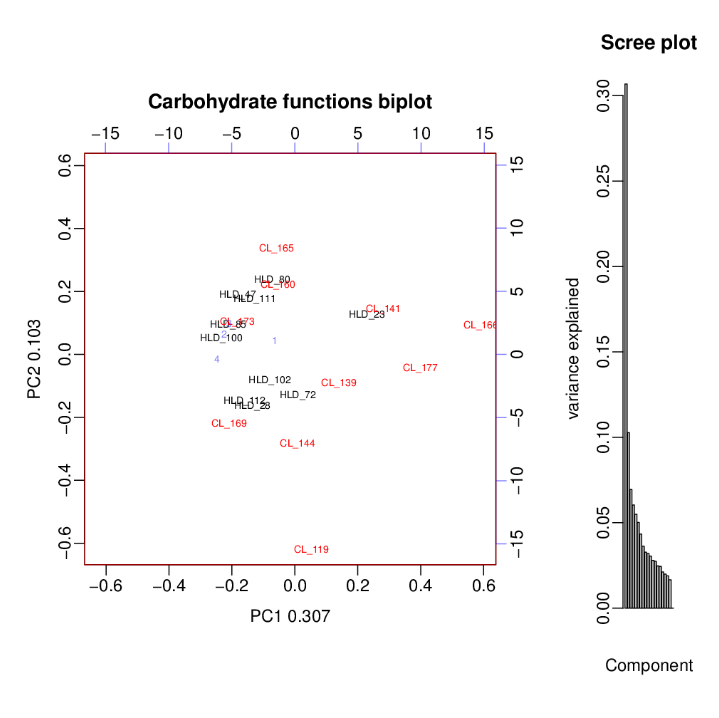
\includegraphics[width=0.95\textwidth]{metagenomic_carb_pca.png}
\caption[Principal components analysis of carbohydrate metagenomic data.]{\textbf{Principal components analysis of carbohydrate metagenomic data.} This biplot shows the sample separation produced when only the 1164 subsystem 4 categories under the `Carbohydrates' subsystem 1 categorization are used. In this biplot, the healthy samples are shown in black, while the extreme NASH samples are shown in red. The location of the subsystem 4 labels (in blue) show which direction they pull the samples in, in terms of variance. The biplot shows only the thirty four subsystem 4 categories with an effect size greater than 1. The Scree plot indicates that about 40\% of the variation in the data set was explained by the first two components, and the data is well spread. Below is the key for the subsystem 4 labels.
\begin{tabular}{|l|l|}
\hline
\bf{Function ID} & \bf{Function name}\\ \hline
1 & Maltodextrin phosphorylase (EC 2.4.1.1) \\ \hline
2 & Dihydrolipoamide acyltransferase component of branched-chain \\
& alpha-keto acid dehydrogenase complex (EC 2.3.1.168) \\ \hline
3 & Predicted L-arabinose isomerase (EC 5.3.1.4) \\ \hline
4 & Predicted galactoside ABC transporter, permease protein 2 \\ \hline
\end{tabular}
}
\label{nafld_metagenomic_carb_pca}
\end{center}
\end{figure}

\begin{figure}[h]
\begin{center}
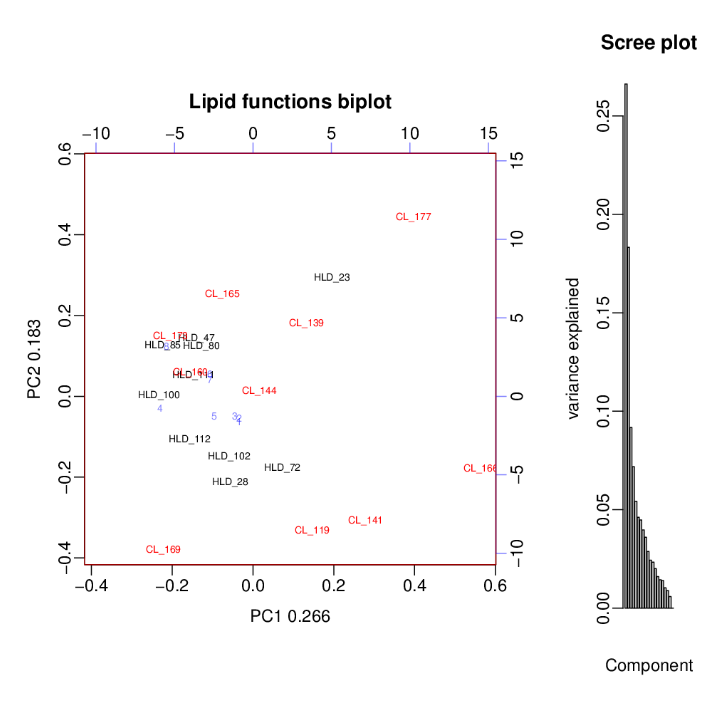
\includegraphics[width=0.95\textwidth]{metagenomic_lipid_pca.png}
\caption[Principal components analysis of lipid metagenomic data.]{\textbf{Principal components analysis of lipid metagenomic data.} This biplot shows the sample separation produced when only the 134 subsystem 4 categories under the `Fatty Acids, Lipids, and Isoprenoids' subsystem 1 categorization are used. In this biplot, the healthy samples are shown in black, while the extreme NASH samples are shown in red. The location of the subsystem 4 labels (in blue) show which direction they pull the samples in, in terms of variance. The biplot shows only the thirty four subsystem 4 categories with an effect size greater than 0.5. The Scree plot indicates that about 40\% of the variation in the data set was explained by the first two components, and the data is well spread. Below is the key for the subsystem 4 labels.
\begin{tabular}{|l|l|}
\hline
\bf{Function ID} & \bf{Function name}\\ \hline
1 & 3-oxoacyl-[acyl-carrier-protein] synthase, KASII (EC 2.3.1.41) \\ \hline
2 & 3-oxoacyl-[acyl-carrier-protein] synthase, KASIII (EC 2.3.1.41) \\ \hline
3 & Acetyl-coenzyme A carboxyl transferase alpha chain (EC 6.4.1.2) \\ \hline
4 & 3-ketoacyl-CoA thiolase (EC 2.3.1.16) \\ \hline
5 & Squalene--hopene cyclase (EC 5.4.99.17) \\ \hline
6 & Hydroxyneurosporene methyltransferase (EC 2.1.1.-) \\ \hline
7 & FIG143263: Glycosyl transferase \\ \hline
8 & Phytoene dehydrogenase and related proteins \\ \hline
\end{tabular}
}
\label{nafld_metagenomic_lipid_pca}
\end{center}
\end{figure}

\begin{figure}[h]
\begin{center}
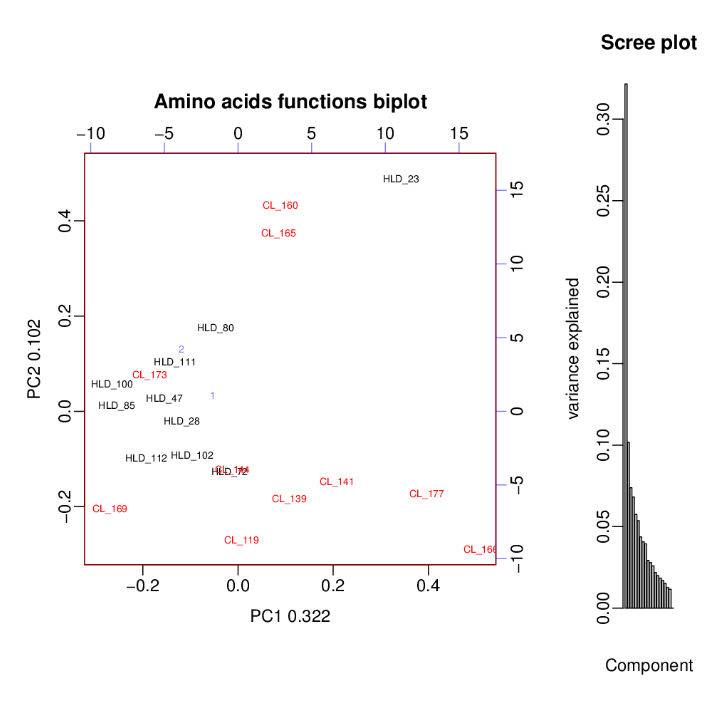
\includegraphics[width=0.95\textwidth]{metagenomic_amino_pca.png}
\caption[Principal components analysis of lipid metagenomic data.]{\textbf{Principal components analysis of lipid metagenomic data.} This biplot shows the sample separation produced when only the 449 subsystem 4 categories under the `Amino Acids and Derivatives' subsystem 1 categorization are used. In this biplot, the healthy samples are shown in black, while the extreme NASH samples are shown in red. The location of the subsystem 4 labels (in blue) show which direction they pull the samples in, in terms of variance. The biplot shows only the thirty four subsystem 4 categories with an effect size greater than 1. The Scree plot indicates that about 40\% of the variation in the data set was explained by the first two components, and the data is well spread. Below is the key for the subsystem 4 labels.
\begin{tabular}{|l|l|}
\hline
\bf{Function ID} & \bf{Function name}\\ \hline
1 & Phosphoadenylyl-sulfate reductase [thioredoxin] (EC 1.8.4.8) \\ \hline
2 & 2,3-diketo-5-methylthiopentyl-1-phosphate enolase \\ \hline
\end{tabular}
}
\label{nafld_metagenomic_amino_pca}
\end{center}
\end{figure}

\FloatBarrier

\paragraph{MetaPhlAn}\mbox{}\\
We ran the sequences from the metagenomic sequencing experiment through MetaPhlAn to examine if the taxonomic profile derived from the metagenomic sequences was similar to the taxonomic profile we measured. MetaPhlAn generates taxonomy profiles that can be compared to the results of 16S rRNA gene tag sequencing.

The operational taxonomic units in the MetaPhlAn and 16S rRNA gene analysis were derived from different databases, and can not be compared directly. Note that OTUs can reside in between genera, such that the genus classification is not perfectly concordant between the two comparisons. The top four relatively abundant genera from the MetaPhlAn analysis were \textit{Ruminococcus}, \textit{Eubacterium}, \textit{Coprococcus}, and \textit{Bacteroides}. \textit{Ruminococcus} \textit{Coprococcus} are also on the top four relatively abundant genera from the 16S rRNA gene tag sequencing experiment.

Figure ~\ref{nafld_metaphlan_barplot} shows the taxonomic composition of each sample, as calculated by MetaPhlAn. The healthy and the extreme NASH samples are not separated by unsupervised clustering, as shown in the dendrogram.

In the ALDEx analysis of differential abundance for each taxa (Figure ~\ref{nafld_metaphlan_aldex}), \textit{Alistipes shahii} was the most differentially abundant (although not significantly so). Other members of the \textit{Alistipes} genus were identified as having top decile effect sizes for relative abundance in the healthy condition in the 16S rRNA gene sequencing experiment, as shown in supporting figure ~\ref{nafld_bot_otu_table}. The OTUs from the 16S rRNA gene sequencing experiment and the taxa in the MetaPhlAn analysis cannot be mapped to each other directly, but it is possible that some members of the 16S OTUs may have genes grouped under \textit{Alistipes shahii} in the MetaPhlAn analysis. Note that one cannot infer information about a bacterial species from the analysis of a bacterial genus, or vice versa, due to the ecological paradox: Inferences cannot be made about members of a group based on the group as a whole.

\begin{figure}[h]
\begin{center}
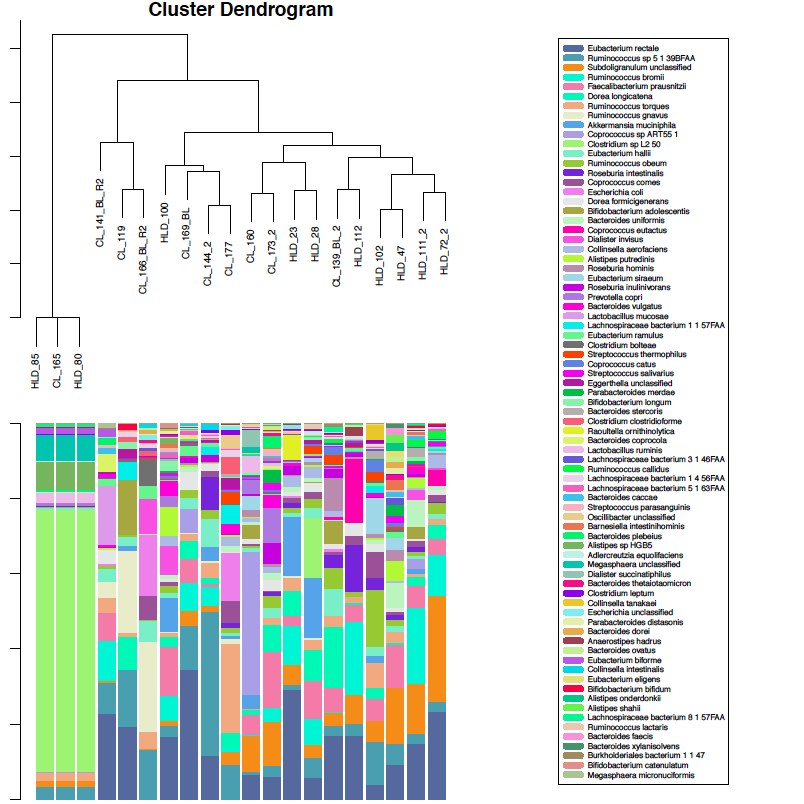
\includegraphics[width=0.95\textwidth]{metaphlan_barplot_dendogram.png}
\caption[Taxa barplot dendogram derived from MetaPhlAn.]{\textbf{Taxa barplot dendogram derived from MetaPhlAn.} The metagenomic reads were input into MetaPhlAn to generate a count table. The taxa in the count table were filtered such that only taxa with at least 1\% abundance in any sample was kept. In this barplot, each bar represents one sample, and each color represents one genus, with the size of the colored segments corresponding with the relative abundance of the genus.}
\label{nafld_metaphlan_barplot}
\end{center}
\end{figure}

\begin{figure}[h]
\begin{center}
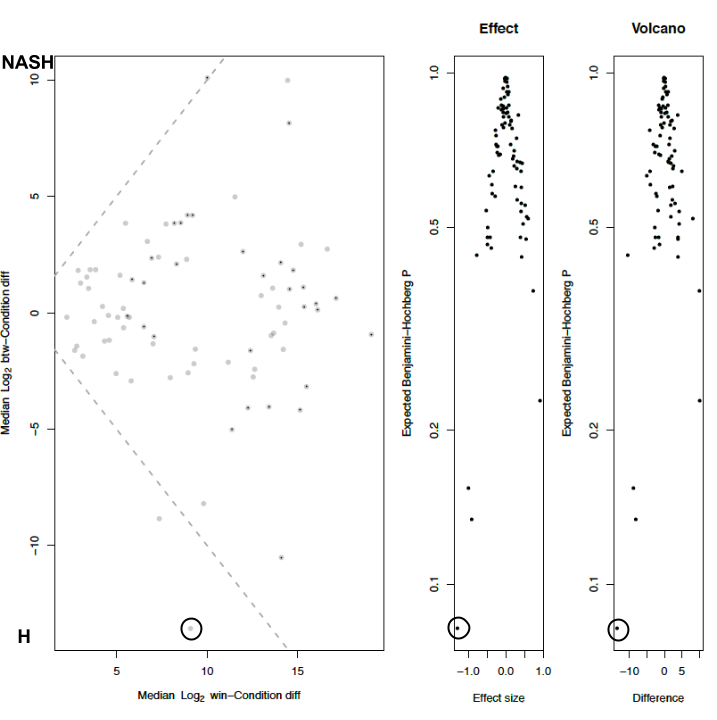
\includegraphics[width=0.95\textwidth]{metaphlan_aldex.png}
\caption[Difference within groups vs. difference between groups per taxa, derived from MetaPhlAn.]{\textbf{Difference within groups vs. difference between groups per taxa, derived from MetaPhlAn.} This plot was generated from the count table inferred by MetaPhlAn, with taxa filtered such that only taxa with at least 1\% abundance in any sample was kept. No taxa are more differential between groups than within groups. A positive difference between indicates that the taxa was relatively increased in NASH while a negative difference between indicates that the taxa was relatively increased in healthy. This analysis was done at the inferred species level (using operational taxonomic units) rather than at the genus level. The circled taxa is \textit{Alistipes shahii}, and has an expected Benjamini-Hochberg p-value of 0.078, and an effect size of -1.25.}
\label{nafld_metaphlan_aldex}
\end{center}
\end{figure}



\FloatBarrier

\section{Discussion}

Given the inconsistency in the five papers that have been published about NAFLD and the gut microbiome, we have performed our analysis in a more statistically rigorous manner in an effort to find OTUs with effects more likely to be consistent across experiments. We found that there was no significant difference between groups by sample clustering (Fig\. ~\ref{nafld_16s_barplot}) or at the level of the individual OTUs (Fig\. ~\ref{nafld_fig3}). The metagenomic data was used to impute taxonomic profiles through MetaPhlAn. In the MetaPhlAn analysis, one taxa, \textit{Alistipes shahii}, was nearly significantly increased in the healthy condition in the MetaPhlAn analysis, which infers a taxonomic profile from metagenomic sequencing. However, when we sequenced the true taxonomic profile through 16S rRNA gene sequencing, no taxa were as differential (Fig. ~\ref{nafld_fig3}), and the groups were not separated (Fig. ~\ref{nafld_16s_biplot}). Members of the \textit{Alistipes} genus appear in the top decile of taxa differentially abundant in both NASH (Fig. ~\ref{nafld_top_otu_table}) and healthy (Fig. ~\ref{nafld_bot_otu_table}) conditions. This suggests that members of the \textit{Alistipes} genus may be a component of the healthy gut microbiome missing in patients with extreme NASH.

We hypothesize that there is a characterizable taxonomic profile difference in the gut microbiome between patients prone to NASH and healthy controls. Further study with an increased sample size, a more homogenous population, and a greater phenotypic difference between groups may provide the statistical power required to detect the nature of this difference. Challenges in obtaining such a data set include cost and recruiting an appropriate population. Model organisms such as mice do not naturally host the same microbiota in their gut as humans \cite{nguyen2015informative}, and it is not known how well a complex human microbiome can colonize a germ free mouse (a process known as `humanization') \cite{clavel2016mouse}. Bacterial communities grown in chemostats also have differences in the proportional abundance of different taxa compared to the fecal matter from which the communities are seeded \cite{mcdonald2013evaluation}. There may be several taxa that differ between the gut microbiomes of healthy patients and patients with extreme NASH. These can be used to develop probiotic or fecal transplant interventions to protect patients at risk against NASH progression.

The study was likely underpowered and there could be several factors that contribute to this. First, the gut microbiome is highly diverse between individuals. This is compounded by the fact that the samples were taken from a diverse Toronto population, including people who immigrated from other countries who likely have different diets. The literature shows that differences in the gut microbiome are often driven by diet \cite{david2014diet}. Additionally, the nature of microbiome data is that there are very many more variables (in the form of OTUs or annotated gene functions) than samples, and the power of the study is inversely proportional to the number of variables.

From Fig\. ~\ref{nafld_fig4}, the correlation shows that even though there is not enough power to detect a significant difference, the difference from the healthy baseline are moving in the same direction through simple steatosis to nonalcoholic steatohepatitis to extreme NASH.

In our metagenomic analysis, we performed a principal component analysis and found that our healthy samples clustered together into two groups (with the exception of one outlier, HLD\_23). The extreme NASH samples were much more spread out. The samples were not arranged this way in the principal component analysis of the 16S rRNA gene experiment. This could be indicative of a core healthy microbiome profile that is more distinguishable by metabolic potential (gene content profile), and potentially by transcriptomic profile, than the taxonomic profile. Rather than deviating from the healthy samples in a specific direction, the microbiome of extreme NASH patients could deviate from the healthy microbiome in a number of directions and yet produce the same clinical outcomes. One other example of this is bacterial vaginosis, which may differ taxonomically from the typical lactobacillus-dominated microbiome in many different ways, but has a common transcriptomic profile that lead to the same clinical symptoms \cite{macklaim2013comparative}.

The gut microbiome of NASH patients are individually difficult to distinguish from the gut microbiome of healthy patients. The dysbiosis associated with NASH is unpredictable as the NASH samples are collectively highly variable. This is supported by the principal components plot showing the variance of the samples in Figure ~\ref{nafld_metagenomic_pca_no_outliers}.

Boursier et al. \cite{boursier2016severity} imputed a metagenomic analysis with PICRUSt \cite{langille2013predictive}, and found significantly differentially abundant functional annotations in KEGG pathways for carbohydrate, lipid, and amino acid metabolism. However, this group did not perform a multiple test correction, and their results cannot be distinguished from false positives. Furthermore, PICRUSt is known to correlate with actual metagenomic results with a Spearman correlation coefficient of approximately 0.7. It is unknown how the extreme differential features identified in PICRUSt behave specifically, compared to a sequenced metagenome.

We performed the metagenomic experiment with principal component analysis on the full set of functional annotations, and subsets of annotations categorized under carbohydrate, lipid, and amino acid. We found that the carbohydrate subset and the lipid subset spread out the samples in a pattern closer to that of the full set of functional annotations, compared to the amino acid subset. This makes sense for the carbohydrate subset which contains over one seventh of all the functional annotations. However, the amino acid subset actually contains several times more annotations (449) compared to the lipid subset (134). Even so, the analysis of the amino acid subset (Figure ~\ref{nafld_metagenomic_amino_pca}) showed higher diversity in the samples from patients with extreme NASH than in the samples from healthy controls, corresponding with the carbohydrate and lipid subsets, as well as the full analysis.

The next step in exploring the relationship between the gut microbiome and non alcoholic fatty liver disease progression is to perform studies with a more homogenous population that have more extreme phenotypic differences, and to include transcriptomic as well as metagenomic experiments. Additionally, we implore other research groups to employ multiple test corrections. This process is meant to reduce the probability of identifying differentially abundant features that are false positives, and omitting this step renders the statistical analysis invalid. A renewed focus on producing rigorous research in the field is necessary for microbiome results, such as those published about non alcoholic fatty liver disease, to be consistently replicable.

\section*{{Supporting Information}}

%DIF >  Include only the SI item label in the paragraph heading. Use the \nameref{label} command to cite SI items in the text.
\begin{figure}[h]
\paragraph*{S1 Fig.}{\mbox{}}\\
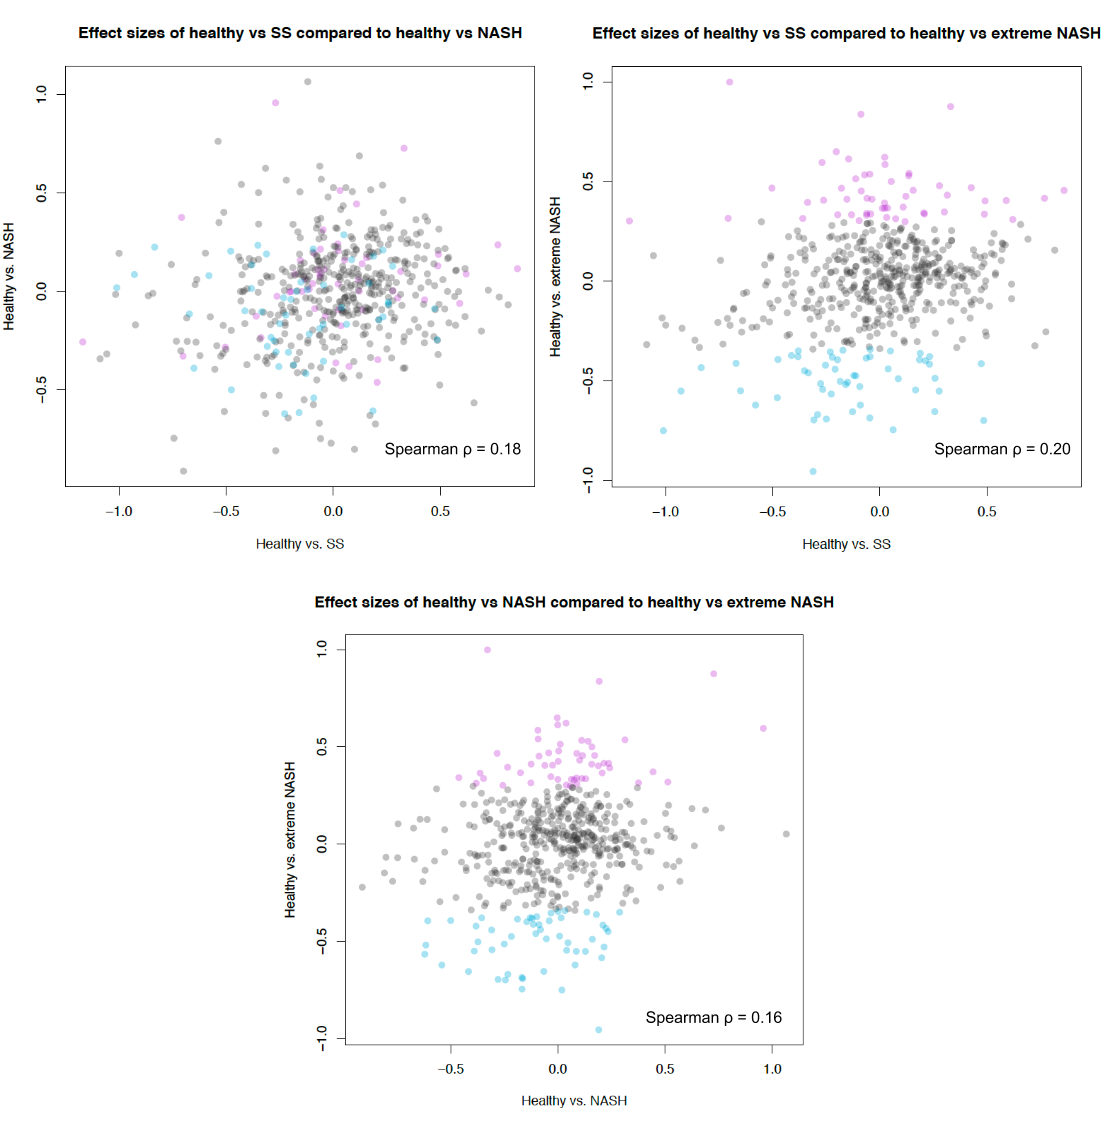
\includegraphics[width=0.9\textwidth]{nafld_16s_effect_sizes_partitioned_healthy.png}
\caption[NAFLD comparison effect sizes, with non overlapping healthy samples.]{{\bf {NAFLD comparison effect sizes, with non overlapping healthy samples.}} In these plots, the healthy and extreme NASH comparison is the same as in Figure ~\ref{nafld_fig4}. To show what the correlations look like without the spurious correlation effects of overlapping samples, the healthy samples not used in the healthy vs. extreme NASH comparison have been partitioned between the healthy vs. SS and the healthy vs. NASH comparison. Additionally, only the NASH samples not used in the extreme NASH comparison are used in the NASH comparison. This way none of the comparisons have overlapping samples.}
\label{nafld_non_overlapping_16s_effect}
\end{figure}


\begin{table}[!ht]
\paragraph*{S2 Fig.}{\mbox{}}\\
% \begin{adjustwidth}{-2.25in}{0in} % Comment out/remove adjustwidth environment if table fits in text column.
\begin{tiny}
\begin{tabular}{|l|l|l|l|l|l|l|l|}
\hline
\bf{OTU family} & \bf{OTU genus} & \bf{SILVA} &\bf{H Vs. SS} & \bf{H Vs. NASH} & \bf{H vs. extreme} \\
& & \bf{bootstrap} & \bf{effect sizes} & \bf{effect sizes} & \bf{NASH effect} \\
& & \bf{value} & & & \bf{sizes}\\ \hline
Acidaminococcaceae & Phascolarctobacterium & 100 & $-0.318$ & $0.043$ & $0.953$ \\ \hline
Lactobacillaceae & Lactobacillus & 97 & $0.479$ & $0.591$ & $0.898$ \\ \hline
Prevotellaceae & Paraprevotella & 100 & $0.048$ & $0.328$ & $0.835$ \\ \hline
Lachnospiraceae & Incertae_Sedis & 98 & $0.25$ & $0.149$ & $0.642$ \\ \hline
Lachnospiraceae & Marvinbryantia & 77 & $0.02$ & $0.164$ & $0.618$ \\ \hline
Ruminococcaceae & Incertae_Sedis & 72 & $0.232$ & $0.31$ & $0.616$ \\ \hline
Bifidobacteriaceae & Bifidobacterium & 100 & $0.064$ & $0.497$ & $0.615$ \\ \hline
Lachnospiraceae & Incertae_Sedis & 73 & $0.218$ & $0.078$ & $0.596$ \\ \hline
Lachnospiraceae & unclassified & 100 & $0.159$ & $0.151$ & $0.564$ \\ \hline
Coriobacteriaceae & unclassified & 97 & $0.17$ & $0.187$ & $0.525$ \\ \hline
Ruminococcaceae & Butyricicoccus & 71 & $0.119$ & $0.236$ & $0.511$ \\ \hline
Lachnospiraceae & unclassified & 98 & $0.246$ & $0.229$ & $0.501$ \\ \hline
Ruminococcaceae & Ruminococcus & 93 & $0.229$ & $0.233$ & $0.497$ \\ \hline
Lachnospiraceae & Incertae_Sedis & 91 & $-0.494$ & $-0.019$ & $0.493$ \\ \hline
Prevotellaceae & Paraprevotella & 100 & $0.126$ & $0.279$ & $0.488$ \\ \hline
unclassified & unclassified & 72 & $0.022$ & $0.181$ & $0.485$ \\ \hline
Ruminococcaceae & unclassified & 100 & $0.817$ & $0.288$ & $0.462$ \\ \hline
Ruminococcaceae & Subdoligranulum & 87 & $0.395$ & $0.141$ & $0.455$ \\ \hline
Ruminococcaceae & Incertae_Sedis & 99 & $0.115$ & $0.025$ & $0.45$ \\ \hline
Prevotellaceae & unclassified & 70 & $0.111$ & $0.156$ & $0.442$ \\ \hline
Lachnospiraceae & unclassified & 100 & $0.202$ & $0.151$ & $0.438$ \\ \hline
unclassified & unclassified & 92 & $0.191$ & $0.287$ & $0.437$ \\ \hline
Coriobacteriaceae & Olsenella & 91 & $0.461$ & $0.236$ & $0.437$ \\ \hline
Lactobacillaceae & Lactobacillus & 98 & $0.103$ & $0.089$ & $0.436$ \\ \hline
Ruminococcaceae & Subdoligranulum & 98 & $0.694$ & $0.274$ & $0.436$ \\ \hline
Ruminococcaceae & Incertae_Sedis & 98 & $0.046$ & $0.112$ & $0.425$ \\ \hline
unclassified & unclassified & 73 & $-0.036$ & $0.009$ & $0.413$ \\ \hline
Prevotellaceae & Prevotella & 99 & $0.234$ & $0.296$ & $0.403$ \\ \hline
Family_XIII & Incertae_Sedis & 100 & $0.036$ & $0.058$ & $0.398$ \\ \hline
Lachnospiraceae & Anaerostipes & 100 & $0.066$ & $-0.177$ & $0.385$ \\ \hline
Ruminococcaceae & Faecalibacterium & 100 & $0.364$ & $0.283$ & $0.374$ \\ \hline
Ruminococcaceae & Ruminococcus & 100 & $0.071$ & $0.091$ & $0.372$ \\ \hline
unclassified & unclassified & 98 & $0.208$ & $0.131$ & $0.367$ \\ \hline
Lachnospiraceae & unclassified & 100 & $0.007$ & $0.192$ & $0.362$ \\ \hline
Bacteroidaceae & Bacteroides & 100 & $-0.064$ & $0.069$ & $0.356$ \\ \hline
Lachnospiraceae & Incertae_Sedis & 100 & $-0.045$ & $0.147$ & $0.355$ \\ \hline
Coriobacteriaceae & Enterorhabdus & 72 & $0.292$ & $0.325$ & $0.345$ \\ \hline
Alcaligenaceae & Sutterella & 100 & $0.057$ & $0.256$ & $0.342$ \\ \hline
Lachnospiraceae & unclassified & 100 & $0.085$ & $0.144$ & $0.339$ \\ \hline
Desulfovibrionaceae & Desulfovibrio & 100 & $0.056$ & $0.269$ & $0.336$ \\ \hline
Rikenellaceae & Alistipes & 100 & $-0.037$ & $0.135$ & $0.332$ \\ \hline
Ruminococcaceae & Subdoligranulum & 92 & $0.469$ & $0.263$ & $0.332$ \\ \hline
Ruminococcaceae & unclassified & 100 & $-0.625$ & $-0.181$ & $0.33$ \\ \hline
Lachnospiraceae & Roseburia & 98 & $-0.353$ & $0.198$ & $0.329$ \\ \hline
Christensenellaceae & unclassified & 99 & $-0.06$ & $0.056$ & $0.328$ \\ \hline
Lachnospiraceae & unclassified & 100 & $0.002$ & $0.145$ & $0.322$ \\ \hline
Veillonellaceae & Dialister & 100 & $0.158$ & $0.355$ & $0.321$ \\ \hline
Lachnospiraceae & Blautia & 97 & $0.13$ & $0.025$ & $0.319$ \\ \hline
Alcaligenaceae & Parasutterella & 100 & $0.089$ & $0.224$ & $0.316$ \\ \hline
Lachnospiraceae & Roseburia & 71 & $-0.016$ & $0.052$ & $0.312$ \\ \hline
Lachnospiraceae & Blautia & 96 & $0.207$ & $-0.056$ & $0.311$ \\ \hline
Pasteurellaceae & unclassified & 100 & $0.094$ & $0.174$ & $0.309$ \\ \hline
Lachnospiraceae & unclassified & 100 & $0.12$ & $-0.004$ & $0.303$ \\ \hline
\end{tabular}
\end{tiny}
\caption[Top decile of OTUs relatively increased in NASH based on effect size from healthy vs. NASH comparison.]{ \textbf{Top decile of OTUs relatively increased in NASH based on effect size from healthy vs. NASH comparison.} This table lists the OTUs and their effect sizes in all the comparisons. The OTUs were picked by open reference, by clustering and comparison with the SILVA database \cite{quast2013silva}. Positive effect sizes indicate that the feature was found to be relatively increased in NASH while negative effect sizes indicate that the feature was found to be relatively increased in healthy. OTUs were annotated with SILVA, and a confidence percentage is reported based on the provided bootstrapping algorithm.}
\label{nafld_top_otu_table}
% \end{adjustwidth}
\end{table}


\begin{table}[!ht]
\paragraph*{S3 Fig.}{\mbox{}}\\
% \begin{adjustwidth}{-2.25in}{0in} % Comment out/remove adjustwidth environment if table fits in text column.
\begin{tiny}
\begin{tabular}{|l|l|l|l|l|l|l|l|}
\hline
\bf{OTU family} & \bf{OTU genus} & \bf{SILVA} &\bf{H Vs. SS} & \bf{H Vs. NASH} & \bf{H vs. extreme} \\
& & \bf{bootstrap} & \bf{effect sizes} & \bf{effect sizes} & \bf{NASH effect} \\
& & \bf{value} & & & \bf{sizes}\\ \hline
Lachnospiraceae & unclassified & 100 & $0.324$ & $-0.113$ & $-0.346$ \\ \hline
Ruminococcaceae & Incertae_Sedis & 100 & $-0.028$ & $-0.361$ & $-0.351$ \\ \hline
Porphyromonadaceae & Odoribacter & 100 & $0.16$ & $-0.226$ & $-0.353$ \\ \hline
Ruminococcaceae & unclassified & 100 & $-0.185$ & $-0.276$ & $-0.361$ \\ \hline
Lachnospiraceae & unclassified & 100 & $-0.507$ & $-0.266$ & $-0.362$ \\ \hline
Lachnospiraceae & Roseburia & 83 & $0.031$ & $-0.043$ & $-0.364$ \\ \hline
Christensenellaceae & unclassified & 100 & $-0.008$ & $-0.192$ & $-0.365$ \\ \hline
Lachnospiraceae & Blautia & 91 & $0.061$ & $-0.092$ & $-0.365$ \\ \hline
Verrucomicrobiaceae & Akkermansia & 100 & $-0.049$ & $-0.098$ & $-0.367$ \\ \hline
S24-7 & unclassified & 100 & $0.28$ & $0.129$ & $-0.368$ \\ \hline
Christensenellaceae & unclassified & 98 & $-0.371$ & $-0.332$ & $-0.368$ \\ \hline
Porphyromonadaceae & Parabacteroides & 100 & $-0.2$ & $-0.05$ & $-0.37$ \\ \hline
Lachnospiraceae & Blautia & 93 & $-0.285$ & $-0.248$ & $-0.389$ \\ \hline
Lachnospiraceae & unclassified & 98 & $0.114$ & $-0.014$ & $-0.391$ \\ \hline
Christensenellaceae & unclassified & 100 & $-0.146$ & $-0.256$ & $-0.4$ \\ \hline
Lachnospiraceae & Roseburia & 91 & $-0.323$ & $-0.254$ & $-0.4$ \\ \hline
Lachnospiraceae & Incertae_Sedis & 85 & $-0.091$ & $-0.246$ & $-0.402$ \\ \hline
Lachnospiraceae & Dorea & 100 & $-0.416$ & $-0.201$ & $-0.403$ \\ \hline
Ruminococcaceae & unclassified & 100 & $-0.384$ & $-0.505$ & $-0.409$ \\ \hline
Christensenellaceae & unclassified & 99 & $-0.278$ & $-0.108$ & $-0.417$ \\ \hline
Erysipelotrichaceae & Turicibacter & 100 & $-0.29$ & $-0.234$ & $-0.43$ \\ \hline
Prevotellaceae & Alloprevotella & 100 & $-0.127$ & $-0.03$ & $-0.437$ \\ \hline
Lachnospiraceae & unclassified & 100 & $-0.553$ & $-0.282$ & $-0.441$ \\ \hline
Ruminococcaceae & Incertae_Sedis & 84 & $-0.129$ & $-0.272$ & $-0.443$ \\ \hline
Porphyromonadaceae & Odoribacter & 100 & $-0.382$ & $-0.303$ & $-0.445$ \\ \hline
Family_XIII & Anaerovorax & 91 & $-0.317$ & $-0.322$ & $-0.447$ \\ \hline
Lachnospiraceae & Incertae_Sedis & 82 & $-0.078$ & $-0.434$ & $-0.451$ \\ \hline
Ruminococcaceae & Ruminococcus & 100 & $-0.077$ & $-0.17$ & $-0.457$ \\ \hline
Veillonellaceae & Dialister & 100 & $0.171$ & $-0.162$ & $-0.497$ \\ \hline
Ruminococcaceae & unclassified & 76 & $-0.373$ & $-0.324$ & $-0.5$ \\ \hline
Rikenellaceae & Alistipes & 100 & $-0.39$ & $-0.219$ & $-0.503$ \\ \hline
Ruminococcaceae & unclassified & 100 & $-0.347$ & $-0.139$ & $-0.518$ \\ \hline
Lachnospiraceae & Blautia & 85 & $-0.413$ & $-0.415$ & $-0.519$ \\ \hline
Coriobacteriaceae & Adlercreutzia & 100 & $0.064$ & $-0.025$ & $-0.525$ \\ \hline
Bacteroidaceae & Bacteroides & 100 & $-0.657$ & $-0.524$ & $-0.526$ \\ \hline
Lachnospiraceae & Pseudobutyrivibrio & 98 & $-0.228$ & $-0.218$ & $-0.531$ \\ \hline
Bacteroidaceae & Bacteroides & 100 & $-0.525$ & $-0.333$ & $-0.536$ \\ \hline
Ruminococcaceae & Faecalibacterium & 100 & $-0.593$ & $-0.402$ & $-0.549$ \\ \hline
Bacteroidaceae & Bacteroides & 100 & $-0.181$ & $0.022$ & $-0.558$ \\ \hline
Bacteroidaceae & Bacteroides & 100 & $-0.398$ & $-0.351$ & $-0.564$ \\ \hline
Bacteroidaceae & Bacteroides & 100 & $-0.39$ & $-0.348$ & $-0.588$ \\ \hline
unclassified & unclassified & 85 & $-0.001$ & $-0.115$ & $-0.589$ \\ \hline
Ruminococcaceae & Incertae_Sedis & 100 & $-0.321$ & $-0.309$ & $-0.636$ \\ \hline
Ruminococcaceae & Subdoligranulum & 99 & $-0.241$ & $-0.386$ & $-0.637$ \\ \hline
Lachnospiraceae & Incertae_Sedis & 85 & $-0.523$ & $-0.404$ & $-0.682$ \\ \hline
Lachnospiraceae & Coprococcus & 91 & $-0.248$ & $-0.304$ & $-0.682$ \\ \hline
Ruminococcaceae & Incertae_Sedis & 97 & $-0.397$ & $-0.415$ & $-0.689$ \\ \hline
Ruminococcaceae & unclassified & 74 & $0.051$ & $-0.193$ & $-0.691$ \\ \hline
Ruminococcaceae & Subdoligranulum & 85 & $-0.251$ & $-0.331$ & $-0.711$ \\ \hline
Ruminococcaceae & Ruminococcus & 100 & $-0.134$ & $-0.15$ & $-0.72$ \\ \hline
Lachnospiraceae & Dorea & 100 & $-0.628$ & $-0.455$ & $-0.731$ \\ \hline
Erysipelotrichaceae & unclassified & 100 & $-0.343$ & $-0.352$ & $-0.754$ \\ \hline
Family_XIII & Incertae_Sedis & 91 & $-0.219$ & $-0.297$ & $-0.93$ \\ \hline
\end{tabular}
\end{tiny}
\caption[Top decile of OTUs relatively increased in healthy based on effect size from healthy vs. NASH comparison.]{ \textbf{Top decile of OTUs relatively increased in healthy based on effect size from healthy vs. NASH comparison.} This table lists the OTUs and their effect sizes in all the comparisons. The OTUs were picked by open reference, by clustering and comparison with the SILVA database \cite{quast2013silva}. Positive effect sizes indicate that the feature was found to be relatively increased in NASH while negative effect sizes indicate that the feature was found to be relatively increased in healthy. OTUs were annotated with SILVA, and a confidence percentage is reported based on the provided bootstrapping algorithm.}
\label{nafld_bot_otu_table}
% \end{adjustwidth}
\end{table}

\begin{figure}[h]
\paragraph*{S4 Fig.}{\mbox{}}\\
\begin{center}
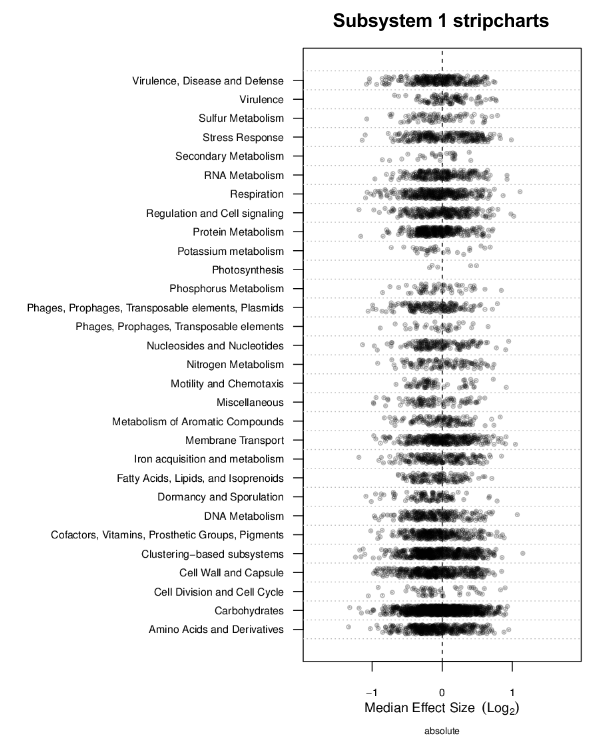
\includegraphics[width=0.95\textwidth]{metagenomic_subsys1.png}
\caption[Difference within vs. difference between healthy and extreme NASH for metagenomic data.]{\textbf{Difference within vs. difference between healthy and extreme NASH for metagenomic data.} Each point on this plot represents a functional annotation at the SEED subsystem 4 level. The different rows of the plots show the subsystem 4 annotations within each subsystem 1 group. Points on the positive side were more abundant in the extreme NASH condition while points on the negative side were more abundant in the healthy condition. None of the points were significantly differentially abundant between groups. In this plot, a large skew of points on one side indicates that a functional category may be more abundant in one condition, but no such large skew exists in this figure.}
\label{nafld_metagenomic_subsys1}
\end{center}
\end{figure}
